%% Submission draft for Journal of Fluids and Structures (Elsevier).
%% Numeric macros come from numbers.tex, generated by scripts/fill_numbers.py.
\documentclass[preprint,11pt,authoryear]{elsarticle}

\usepackage[T1]{fontenc}
\usepackage{lmodern}
\usepackage{amsmath,amssymb,amsthm}
\usepackage{array}
\usepackage{booktabs}
\usepackage{graphicx}
\usepackage{siunitx}
\usepackage{algorithm}
\usepackage{algpseudocode}
\usepackage[hidelinks]{hyperref}
\usepackage[protrusion=true,expansion=false]{microtype}

\newtheorem{proposition}{Proposition}
\newtheorem{remark}{Remark}

\newcommand{\Uf}{U_{\mathrm{f}}}
% Generated by scripts/fill_numbers.py -- do not edit numeric macros by hand.
\newcommand{\FlutterSpeed}{137.35}
\newcommand{\FeasibleCells}{6}
\newcommand{\TotalCells}{9}
\newcommand{\LocalFbStabilised}{4}
\newcommand{\LocalFbHealthy}{-0.03}
\newcommand{\LqrFixedStabilised}{5}
\newcommand{\LqrFixedHealthy}{-5.15}
\newcommand{\LqrSchedStabilised}{5}
\newcommand{\LqrSchedHealthy}{-5.08}
\newcommand{\LqgLocalStabilised}{5}
\newcommand{\LqgLocalHealthy}{-5.52}
\newcommand{\LqrOracleStabilised}{6}
\newcommand{\LqrOracleHealthy}{-5.07}
\newcommand{\CommOracleStabilised}{6}
\newcommand{\CommOracleHealthy}{-0.18}
\newcommand{\IppoPhysicsStabilised}{6}
\newcommand{\IppoPhysicsHealthy}{-0.25}
\newcommand{\MoccaStabilised}{5}
\newcommand{\MoccaHealthy}{-0.14}
\newcommand{\RecurrentOnlyStabilised}{5}
\newcommand{\RecurrentOnlyHealthy}{-0.04}
\newcommand{\BestRobustVariant}{comm\_oracle}
\newcommand{\BestRobustStabilised}{6}
\newcommand{\BestNominalVariant}{ippo\_physics}
\newcommand{\BestNominalHealthy}{-0.25}
\newcommand{\ResultsSummarySentence}{\emph{[ResultsSummarySentence: to be written]}}
\newcommand{\ResultsNarrative}{\emph{[ResultsNarrative: to be written]}}
\newcommand{\ResultsAblations}{\emph{[ResultsAblations: to be written]}}
\newcommand{\PhaseNarrative}{\emph{[PhaseNarrative: to be written]}}
\newcommand{\ConclusionSentence}{\emph{[ConclusionSentence: to be written]}}


\journal{Journal of Fluids and Structures}

\begin{document}

\begin{frontmatter}

\title{A physics-exact credit decomposition for distributed flutter
suppression, and the exploration scale that hides it}

\author[buv]{Quang-Vinh Dang}
\ead{vinh.dq4@buv.edu.vn}
\author[xtech]{Hai Dang Nguyen}
\ead{haidang5101994@gmail.com}
\author[vgu]{Ngoc Minh La}
\ead{lmngocdhsp@gmail.com}
\author[mu]{Minh Ngoc Dinh\corref{cor1}}
\ead{minh.dinh@maeducation.com}

\cortext[cor1]{Corresponding author.}
\affiliation[buv]{organization={British University Vietnam},
                   city={Hung Yen}, country={Vietnam}}
\affiliation[xtech]{organization={XTECH AI Technology},
                     city={Ho Chi Minh City}, country={Vietnam}}
\affiliation[vgu]{organization={Vietnamese German University},
                   city={Ho Chi Minh City}, country={Vietnam}}
\affiliation[mu]{organization={School of Data Science \& Information
                  Technology, Millennia University},
                  city={Ho Chi Minh City}, country={Vietnam}}

\begin{abstract}
Differentiating the aeroelastic energy of a structural plant along its
trajectories isolates a control-power term exactly additive across an
arbitrary number of control inputs. We use this to give multi-agent
reinforcement learning, applied to distributed flutter suppression on several
independently actuated surfaces of a Goland wing cross-validated against an
unsteady vortex-lattice solver, a closed-form per-agent credit signal in place
of the estimated one the method normally requires. Combined with log-energy
shaping, this credit beats the closed form alone ($g=-2.49$, corrected $p=0.020$, also against a
naive reward and an adapted VDN-style baseline); it does not significantly
beat shaping alone at that standard, which a less rigorous earlier version
overstated, and we report the retraction with the finding. Its advantage over the estimated alternatives is reliability, not raw
mean: both match or exceed it on some seeds and fail on others, at higher
variance.

None of this was visible at conventional exploration settings. A controller
achieving the classical result uses \SI{0.105}{\degree} RMS deflection,
against \SI{4.5}{\degree} for a conventional exploration standard deviation;
every mechanism we tried plateaued until exploration was matched to that
amplitude, changing performance by a factor of two and making the credit
result measurable at all. We further checked that the credit's sign tolerates plausible identification
error and that the classical baseline's envelope-edge divergence is not simply
a tuning artefact. The learned policies still trail a decentralised LQG on
average damping ($-1.53$ against $-2.05\,\mathrm{s}^{-1}$) while holding one
condition it cannot, pointing toward a certified-plus-monitored-residual
architecture we have not yet built.
\end{abstract}

\begin{keyword}
active flutter suppression \sep aeroelasticity \sep multi-agent reinforcement
learning \sep credit assignment \sep decentralised control \sep exploration
\end{keyword}

\end{frontmatter}

\section*{Nomenclature}
\begin{tabular}{@{}lp{10.2cm}@{}}
$q,\dot q,\ddot q$ & modal coordinates, rates, accelerations \\
$M,C,K$ & modal mass, damping, stiffness matrices \\
$L,x_{\mathrm{w}}$ & wake-coupling matrix and wake (Wagner lag) states \\
$B,\delta,b_k$ & control-influence matrix, deflection vector, its $k$th column \\
$E$ & instantaneous structural energy, $\tfrac12\dot q^\top M\dot q+\tfrac12 q^\top Kq$ \\
$P_k$ & control power of agent $k$, $(\dot q^\top b_k)\delta_k$ \\
$\lambda$ & energy decay rate, $\tfrac12\,\mathrm{d}(\log E)/\mathrm{d}t$ \\
$D_k$ & difference reward for agent $k$ \\
$U,\Uf$ & airspeed, flutter speed \\
$N$ & number of control surfaces / agents \\
$R$ & number of retained modal phasors ($R{=}2$ throughout) \\
$o_k,a_k$ & agent $k$'s local observation and normalised action \\
$\hat\phi_k$ & agent $k$'s encoded phasor estimate, $\in\mathbb{R}^{2R}$ \\
$e_k$ & consensus message received by agent $k$ \\
$\sigma$ & initial policy exploration standard deviation (normalised action units) \\
$d,p$ & Cohen's $d$ effect size, Welch's $t$-test $p$-value \\
\end{tabular}

\section{Introduction}
\label{sec:intro}

Flutter is a self-excited aeroelastic instability in which structural bending and
torsion couple through unsteady aerodynamic loads and draw energy from the
freestream. Past a critical speed the coupled mode becomes unstable and the
response grows without bound, typically within a few oscillation cycles and with
no warning a pilot can act on. It has been a design driver since the earliest
flexible aircraft and remains one: because a wing must be certified against
flutter with a substantial speed margin, the mass, stiffness and manufacturing
cost of the structure are set in large part by an instability the aircraft is
never meant to encounter in service \citep{livne2018flutter,
mukhopadhyay2003historical}. Active suppression offers a way to buy back some of
that margin with control effort rather than with structural weight, which is why
it has attracted sustained engineering attention since the 1970s
\citep{karpel1982design,waszak2001robust,block1998applied}.

Two trends motivate revisiting the problem now. First, wings are becoming more
flexible --- for fuel efficiency, span, and load alleviation --- and flexible
wings carry more independently actuated trailing-edge surfaces, each with its own
local sensing and local computation on a bus rather than a dedicated wire to a
central controller. The hardware is already distributed even where the control
law is not. Second, reinforcement learning has been applied to flutter
suppression with encouraging results: circulation control validated in a wind
tunnel \citep{circulation2023}, camber morphing for stall flutter
\citep{stallflutter2025}, and tuning the parameters of a conventional controller
\citep{flyingwing2022}. Every instance we are aware of, however, uses a single
agent commanding a single effector from a global observation. Taking the
hardware trend seriously means asking what happens when the effectors are
commanded by separate agents that cannot see the whole wing, which is the
question this paper answers on a specific, validated testbed
(Figure~\ref{fig:schematic}).

Posing the problem with one agent per surface makes credit assignment the central
difficulty, and for a physical reason rather than an algorithmic one: every
surface acts on the \emph{same} coupled bending--torsion mode, so a reward built
from the whole wing's response says almost nothing about which surface actually
helped. The standard remedies in multi-agent reinforcement learning estimate that
decomposition statistically, from the returns a policy happens to collect
\citep{sunehag2018vdn,rashid2018qmix,foerster2018coma}. Our first observation is
that this particular class of plant does not require estimation at all: for a
structural system whose energy budget is exactly additive across control inputs,
the credit decomposition is available in closed form from the equations of
motion themselves, with no learning involved in computing it.

Our second observation is the one we would most want a practitioner to take away,
and we did not anticipate it going in. Before finding it, we spent several
rounds comparing credit signals, communication schemes, action
parameterisations, recurrence and auxiliary losses --- the ordinary methodology
of an ablation study --- and every variant plateaued in the same narrow
performance band regardless of which mechanism it used. That invariance was not
evidence that the mechanisms were equivalent to one another; on closer
inspection it was evidence that something \emph{upstream} of all of them was
binding. The exploration standard deviation of the policy was roughly forty
times the deflection amplitude that actually damps this wing, so no policy ever
experienced the fine, precisely-phased actuation that works, and no credit
signal --- however well constructed --- could assign credit to a signal buried
that far under noise. Matching the exploration scale to the useful actuation
amplitude changed performance by a factor of two, more than any single
algorithmic choice we tried, and only after that correction did the
credit-assignment effect we had set out to study become measurable at all.

This is a known failure mode in spirit: the reinforcement learning literature has
repeatedly found implementation and hyperparameter choices dominating
algorithmic ones in general-purpose control benchmarks
\citep{henderson2018matters,engstrom2020implementation,andrychowicz2021what}. Our
contribution is a control-specific instance of that caution, with a diagnostic a
practitioner can use \emph{before} training anything: the useful actuation
amplitude is computable from a classical design, and the exploration scale can be
checked against it in advance rather than discovered by trial and error.

\paragraph{Contributions}
\begin{enumerate}
\item A closed form for the multi-agent difference reward in an
energy-conserving structural plant with additive control authority
(Proposition~\ref{prop:diff}), together with the correction that makes it usable:
the credit must be the logarithmic decay rate, not the raw energy rate
(Section~\ref{sec:log}).
\item A five-variant credit-assignment comparison, corrected for the number of
comparisons made, against a naive undecomposed reward and an adapted
value-decomposition baseline in the style of VDN as well as against each half
of the closed-form-plus-shaping credit alone: the closed-form credit's
advantage over an estimated one is in consistency across seeds and conditions,
not a uniformly larger effect size (Section~\ref{sec:ablations}).
\item A quantified account of what limits learning on this problem, with a
diagnostic a practitioner can apply in advance, and a capability probe that rules
out the competing explanation (Section~\ref{sec:exploration}), together with a
direct check of how much control-influence identification error the credit
signal's sign tolerates (Section~\ref{sec:credit-sensitivity}).
\item A validated testbed and a six-rung classical baseline ladder that
separates the control method from the information structure available to it,
cross-validated against an unsteady vortex-lattice solver, including a check of
whether the classical baseline's fragility at the envelope edge is a tuning
artefact rather than an assumption (Sections~\ref{sec:plant},
\ref{sec:design} and~\ref{sec:robust-baseline}).
\item A negative result reported as such: the communication and action
parameterisation mechanisms we derived from the physics do not help, at a
level of statistical correction that makes the negative result harder to
dismiss rather than easier.
\end{enumerate}

\section{Related work}
\label{sec:related}

\paragraph{Active flutter suppression}
The classical approach synthesises a single centralised regulator from a
state-space aeroelastic model, driving all control surfaces from one observer
and one gain \citep{karpel1982design}. Robust multivariable designs following
that template have been demonstrated on wind-tunnel models
\citep{waszak2001robust}, and the approach extends to nonlinear aeroelastic
structures with limit-cycle behaviour \citep{block1998applied}; Livne
\citep{livne2018flutter} surveys the state of the art and the gap between
laboratory demonstrations and certified hardware, and Mukhopadhyay
\citep{mukhopadhyay2003historical} traces the field's history from Theodorsen's
original frequency-domain analysis to modern aeroservoelastic synthesis. Two
things stand out reading this literature together. First, every design in it is
re-derived for a new airframe: the state-space model, the actuator suite and
the sensor placement all change with the aircraft, and Livne's survey is
explicit that the gap between a laboratory demonstration and certified hardware
is as much about this re-engineering cost as about control-theoretic novelty.
Second, and more consequential for this paper, none of these treatments
questions the centralised structure itself: the regulator sees the whole state
and commands every surface jointly, which is exactly the assumption a
physically distributed set of actuators --- multiple independently wired
trailing-edge surfaces on a modern flexible wing, each with its own local
sensing --- need not satisfy. Karpel's original formulation
\citep{karpel1982design} already treats gust alleviation and flutter
suppression as the same state-feedback problem, and we inherit that framing for
the objective in Section~\ref{sec:problem} even though the control structure we
study departs from it. The unsteady aerodynamic models underlying both the
classical literature and our own plant descend from Theodorsen's
frequency-domain analysis \citep{theodorsen1935} and the indicial
(Wagner-function) formulation of Jones \citep{jones1940}; finite-state
induced-flow models \citep{peters1995finite} are the modern sectional
alternative, extending the same lag-state idea to a richer wake representation
than the two-state approximation we use, and
\citep{fung1955,bisplinghoff1955,palacios2023flexible} are the standard texts we
draw the modelling conventions from, with Palacios and Cesnik
\citep{palacios2023flexible} in particular covering the coupled
flight-mechanics setting our plant deliberately simplifies away from.

\paragraph{Adaptive flutter suppression}
Between the fixed-gain classical designs above and the learned policies of the
next paragraph sits a mature adaptive-control literature aimed at exactly the
gap our own motivation cites --- an aerodynamic model that is never exactly the
design model in flight. Downs and Prazenica \citep{downs2023adaptive} apply
direct adaptive control to a three-dimensional flexible wing with nonlinear
stiffness and actuator freeplay, stabilising post-flutter conditions a
fixed-gain LQR cannot; Mozaffari-Jovin et al.\ \citep{mozaffarijovin2024l1}
design an $\mathcal L_1$ adaptive law for a flapped aeroelastic section under
unmatched nonlinear uncertainty, the same flap-actuated setting we study.
Both retain a single, centralised regulator per airframe and adapt its
parameters online rather than decomposing the effectors into separate agents,
so they answer a different question from the one this paper asks --- robustness
to model error at one control point, rather than what changes when the control
points themselves are separate decision-makers --- and are a closer classical
relative to our problem than the fixed-gain designs above, worth situating
against directly rather than folding into the same paragraph as work that
does not address model uncertainty at all.

\paragraph{Learning for flutter control}
A recent line of work applies deep reinforcement learning directly to flutter
suppression: stall flutter via active camber morphing
\citep{stallflutter2025}, trailing-edge circulation control validated in a wind
tunnel \citep{circulation2023}, and tuning the parameters of a conventional
aeroservoelastic controller \citep{flyingwing2022}. The appeal of learning here
is specific to the problem, not generic: flutter is a nonlinear instability once
the response leaves the small-perturbation regime the classical model is valid
in, the aerodynamic model available in flight is never exactly the design model,
and a policy that has seen a distribution of conditions in simulation can in
principle interpolate across off-nominal cases a fixed gain cannot. Despite
using different effectors and different plants, the three studies above share
the same structural assumption as the classical literature they replace a
hand-designed gain in: one learning agent, one effector, one global observation.
None asks what changes when the effectors are commanded by separate agents that
cannot see the whole wing, which is the question a wing with several
independently actuated surfaces on a shared bus makes practically relevant and
is the gap this paper occupies. Framing a wing's own surface as a multi-agent
system is not without precedent: Shalymov et al.\
\citep{shalymov2020feathers} cover an entire wing in many small independently
actuated ``feathers'' and synthesise a speed-gradient adaptive control law
across them, which is multi-agent \emph{control} in the classical sense. What
we are not aware of is prior work that trains separate \emph{learning} agents,
each with only its own local, partial observation of the plant, to solve this
problem --- the distinction that matters here, since the entire credit-assignment
question this paper poses (Section~\ref{sec:related}, ``Multi-agent credit
assignment'') only arises once each surface's controller is estimated from
experience under partial observability rather than derived, as in
\citep{shalymov2020feathers}, from a single control law with access to the
whole system's dynamics.

\paragraph{Decentralised control}
That decentralisation costs closed-loop performance relative to a centralised
design with the same model is a classical result, not a symptom of using
learning \citep{siljak1991decentralized,bakule2008decentralized}. Bakule's
survey \citep{bakule2008decentralized} catalogues exactly the design patterns
this paper's baseline ladder instantiates --- decentralised state feedback with
no inter-subsystem model, and decentralised observers each estimating only a
local state --- and reports the same qualitative cost of decentralisation across
a wide range of application domains, well outside aeroelasticity. The
structural conditions under which decentralised synthesis remains
\emph{tractable} at all, rather than merely stable, are characterised by
Rotkowitz and Lall \citep{rotkowitz2006characterization}: convex synthesis
survives decentralisation exactly when the information structure is
\emph{quadratically invariant} with respect to the plant, a condition our
line-graph sensing pattern does not satisfy in general, which is part of why
the fully decentralised LQG of \ref{app:baselines} is synthesised
independently per surface rather than as a single convex program. This
literature is why we treat the information structure as an experimental
variable rather than an afterthought: comparing a distributed learned policy
against a centralised regulator conflates the control method with the
information available to it, and the honest classical baseline for a policy
that sees only local accelerometers is a fully decentralised LQG built from the
same sensing, not the centralised design that the learned policy could never in
principle match.

\paragraph{Multi-agent credit assignment}
The standard tools for the credit-assignment problem we pose are difference
rewards \citep{wolpert2002difference} and learned value factorisation
\citep{sunehag2018vdn,rashid2018qmix}, with COMA \citep{foerster2018coma} using a
counterfactual advantage baseline to the same end; MADDPG
\citep{lowe2017maddpg} and MAPPO \citep{yu2022mappo} are the common actor-critic
baselines built on top of these ideas, the field more broadly is surveyed in
\citep{albrecht2023survey,scalingmarl2025}, and estimators continue to be
refined \citep{multilevelcredit2025}. These methods differ in how much they
assume about the environment, but all of them estimate the credit
decomposition statistically, from returns a policy happens to collect: VDN and
QMIX \citep{sunehag2018vdn,rashid2018qmix} learn a factorisation of a joint
value function, COMA \citep{foerster2018coma} learns a counterfactual baseline
by marginalising a learned critic over one agent's action, and the original
difference-reward formulation \citep{wolpert2002difference} itself typically
requires a counterfactual rollout with the agent of interest removed. All of
this machinery exists \emph{because} the environment is treated as a black box.
Our contribution is narrower and complementary rather than competing with this
literature: for the specific class of energy-conserving structural plant
studied here, the decomposition these methods estimate is available in closed
form directly from the equations of motion (Proposition~\ref{prop:diff}), with
no learning, no counterfactual rollout and no critic involved in computing it.
We see this less as a competitor to the general-purpose methods above than as
evidence that physical structure, where it exists, is worth exploiting before
reaching for a general estimator built to work without it. The formal setting
for the distributed problem itself is the decentralised POMDP
\citep{bernstein2002complexity,oliehoek2016concise}, whose complexity results
motivate treating partial observability as intrinsic to the sensing
architecture (Section~\ref{sec:problem}) rather than as a modelling
simplification to be relaxed.

\paragraph{Learned communication}
CommNet \citep{sukhbaatar2016commnet} and TarMAC \citep{das2019tarmac} learn
message content end to end from a broad channel, with TarMAC additionally
learning \emph{who} to attend to via a signature-based attention mechanism over
neighbours. We took the opposite design choice on both counts: message
\emph{content} is fixed to a modal phasor derived from the physics rather than
learned end to end, and message \emph{routing} is fixed to the spanwise line
graph rather than learned, on the reasoning that this would make the channel
interpretable and bound its bandwidth independently of the number of agents ---
a property that matters on a physical avionics bus in a way it does not in the
simulated coordination games this literature is usually evaluated on. Measured
against a plain policy with no channel at all, neither the fixed content nor
the fixed routing helped on this plant (Section~\ref{sec:ablations}), and we
report the negative result rather than omit the mechanism; Section~\ref{sec:discussion}
returns to what we think this does and does not say about learned communication
more broadly.

\paragraph{Multi-agent benchmarks and physical grounding}
The environment in this paper is implemented against the PettingZoo
parallel-environment API \citep{terry2021pettingzoo}, the standard interface
much of the multi-agent reinforcement learning literature above is evaluated
through, including the particle-world benchmarks introduced alongside MADDPG
\citep{lowe2017maddpg}. That shared interface is deliberate: it is what lets
the credit-assignment and communication mechanisms surveyed above be dropped
into this environment largely unmodified, which is what makes the ablations of
Section~\ref{sec:ablations} a fair test of those mechanisms rather than a test
of our own re-implementation of them. Where this environment differs from the
particle-world and grid-world benchmarks that dominate the credit-assignment
literature is that its dynamics are not designed for the coordination problem
they pose; they are a validated model of a physical instability
(Section~\ref{sec:plant}), and the credit structure in
Proposition~\ref{prop:diff} is a property of that physics rather than of the
environment's authorial choices. We think this is a meaningful axis along
which physically-grounded multi-agent control tasks are currently
under-represented relative to abstract coordination games, and offer this
testbed as one instance of closing that gap rather than as a claim that
abstract benchmarks are not useful for what they are designed to measure.

\paragraph{Reinforcement learning practice}
Our central caution has direct precedent in general-purpose reinforcement
learning, though not, to our knowledge, applied to a physical control problem
where the binding quantity can be predicted in advance. Henderson et al.\
\citep{henderson2018matters} documented how seed-to-seed variance can swamp the
algorithmic differences a paper sets out to measure; Engstrom et al.\
\citep{engstrom2020implementation} showed that implementation details, not the
nominal algorithm, accounted for much of PPO's reported advantage over TRPO;
Andrychowicz et al.\ \citep{andrychowicz2021what} found hyperparameters
dominating architectural choices at scale; and Agarwal et al.\
\citep{agarwal2021precipice} argued for reporting effect sizes and uncertainty
rather than point estimates from few runs, a practice we follow throughout
Section~\ref{sec:ablations}. Yu et al.\ \citep{yu2022mappo} make a related point
specific to the multi-agent setting: much of MAPPO's reported advantage over
more elaborate multi-agent actor-critic methods traces to implementation
details --- value normalisation, advantage standardisation, the choice of
critic input --- rather than to the algorithm's nominal novelty, which is the
multi-agent analogue of Engstrom et al.'s finding and part of why
Section~\ref{sec:architecture} documents our own architecture choices at the
level of individual design decisions rather than only by name. What we add to
this literature is a case in which the dominant hyperparameter --- the
exploration scale --- is not merely discoverable by sweeping it, but
\emph{computable in advance} from a classical design of the same plant, which
is not true of hyperparameters in the general-purpose benchmarks this
literature studies. Residual formulations, in which a learned policy corrects a
fixed classical controller rather than replacing it
\citep{johannink2019residual,silver2018residual}, appear here as one of the
variants we evaluate rather than as the proposed method.

\paragraph{Positioning}
Table~\ref{tab:positioning} summarises the four axes above together, since no
single prior study we are aware of combines more than one of them: multi-agent
treatment of the individual control surfaces of one wing, a credit signal
derived in closed form from the plant's own physics rather than estimated,
validation of the plant itself against a higher-fidelity solver rather than
only against a published linear benchmark, and an explicit, reproducible
account of what a conventional exploration setting hides. Each axis is
individually present somewhere in the literature surveyed above; their
combination, and the negative and cautionary results that combination
surfaces, is what this paper contributes.

\begin{table}[t]
\centering
\caption{This paper against the literature it draws on, along the axes
Section~\ref{sec:related} discusses. A \checkmark marks that the property
holds for the representative citation(s) in that row; \texttt{--} marks that it
does not; \texttt{n/a} marks that the axis does not apply to that line of work
at all (a single-agent or single-regulator method has no multi-agent credit
decomposition to be closed-form \emph{or} estimated, so neither \checkmark nor
\texttt{--} would be meaningful there).}
\label{tab:positioning}
\small
\begin{tabular}{@{}p{4.4cm}ccc@{}}
\toprule
& Multi-agent & Closed-form & Validated against \\
& surfaces & credit & higher-fidelity solver \\
\midrule
Classical AFS \citep{karpel1982design,waszak2001robust} & -- & n/a & varies \\
Adaptive AFS \citep{downs2023adaptive,mozaffarijovin2024l1} & -- & n/a & -- \\
Learned AFS \citep{stallflutter2025,circulation2023,flyingwing2022} & -- & -- & -- \\
General MARL credit \citep{sunehag2018vdn,rashid2018qmix,foerster2018coma} & \checkmark & -- & n/a \\
Residual control \citep{johannink2019residual,silver2018residual} & -- & -- & n/a \\
This paper & \checkmark & \checkmark & \checkmark \\
\bottomrule
\end{tabular}
\end{table}

\section{Problem formulation and plant model}
\label{sec:problem}

\subsection{Decentralised partially observable decision process}

We model the task as a Dec-POMDP \citep{bernstein2002complexity,oliehoek2016concise}
$\langle \mathcal{I}, \mathcal{S}, \{\mathcal{A}_k\}, T, \{\Omega_k\}, O, R,
\gamma \rangle$. The agent set $\mathcal{I}=\{1,\dots,N\}$ has one member per
control surface. The state $s = (q,\dot q, x_{\mathrm{w}}, \delta)$ collects the
modal coordinates, their rates, the wake states and the current deflections.
Agent $k$ chooses a normalised command $a_k \in [-1,1]$, which its actuator
converts to a physical deflection subject to a rate limit and travel stops.

Each agent observes only $o_k \in \Omega_k$: an accelerometer pair at its own
station, local plunge rate, twist and twist rate, its own saturation fraction,
and air data. Crucially $o_k$ does not contain the modal state. The unstable mode
is a global quantity that no single station can measure, so the partial
observability is intrinsic to the physical arrangement rather than an artefact of
our formulation. Communication, where used, is nearest-neighbour along the span.

\subsection{Objective}

We use the standard discounted formulation \citep{sutton2018reinforcement}. The
quantity to be minimised is the exponential growth rate of the structural energy
$E$, which is also the quantity we report:
\begin{equation}
\lambda \;=\; \tfrac{1}{2}\,\frac{\mathrm{d}}{\mathrm{d}t}\log E ,
\label{eq:objective}
\end{equation}
negative when the wing is being damped. Stating the objective this way, rather
than as an accumulated quadratic cost, matters later: it is what allows the
per-agent credit and the evaluation metric to be literally the same quantity
(Section~\ref{sec:log}).

\subsection{Model}
\label{sec:plant}

We use a modally reduced uniform cantilever wing, shown schematically in
Figure~\ref{fig:schematic}. Three trailing-edge surfaces occupy spanwise bands at
$[0.05,0.40]$, $[0.40,0.72]$ and $[0.72,0.98]$ of the semispan (panel a), hinged
at \SI{75}{\percent} chord (panel b), with $\pm\SI{15}{\degree}$ travel,
\SI{200}{\degree\per\second} rate limit and a \SI{20}{\milli\second} first-order
servo lag. Each surface is commanded by its own agent, which observes only a
local accelerometer pair, local plunge and twist rate, its own saturation
fraction, and air data; no agent observes the modal state, and the three agents
share no channel unless a communication mechanism is explicitly under test
(panel c). Control runs at \SI{200}{\hertz}.

\begin{figure}[t]
\centering
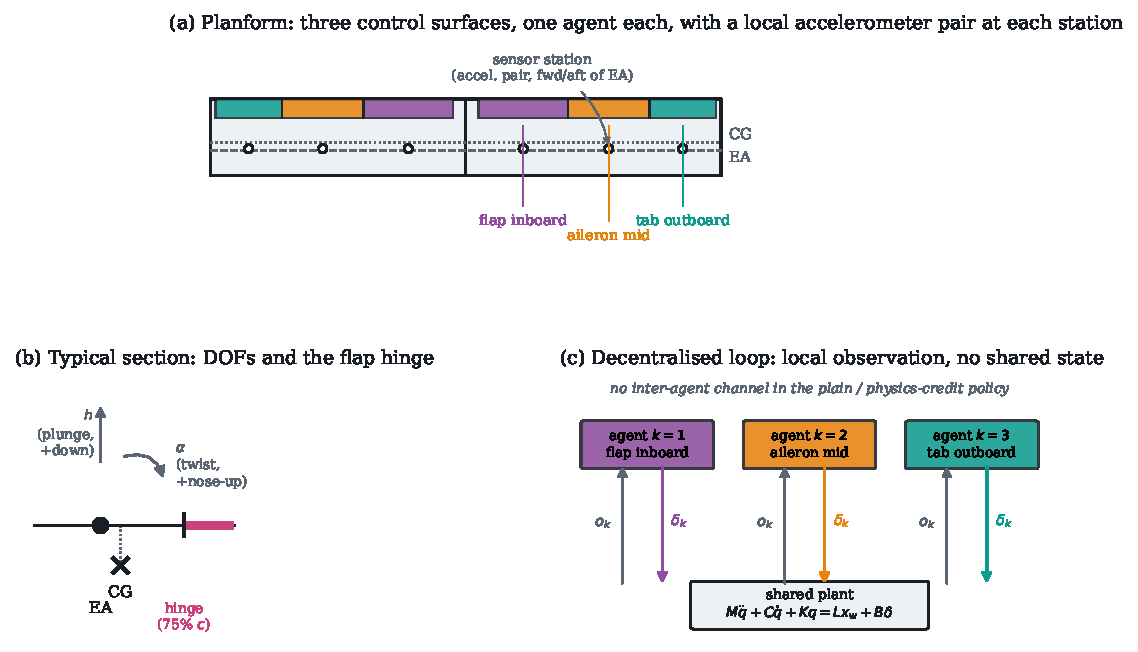
\includegraphics[width=\textwidth]{figures/fig_schematic.pdf}
\caption{The testbed. (a) Planform, agent colours matched throughout the paper.
(b) The typical-section degrees of freedom and the flap hinge that the
thin-airfoil derivative in Section~\ref{sec:sharpy} refers to. (c) The
information structure: each agent closes its own loop through the shared plant,
with no inter-agent channel in the plain and physics-credit policies.}
\label{fig:schematic}
\end{figure}

\subsection{What flutter and its suppression look like}
\label{sec:filmstrip}

Every quantity in the rest of the paper is a scalar derived from a wing that is
physically bending and twisting, and it is worth seeing that motion once before
reducing it to decay rates. Figure~\ref{fig:filmstrip} gives the same initial
\SI{5}{\centi\metre} tip pluck two treatments at $U/\Uf=1.10$, six shared
instants apart, on one shared deformation scale so a flat-looking row is not an
axis artefact. Left to right along the top row is exactly what ``flutter''
names: bending and torsion lock into a fixed phase relationship and the
response grows, visibly, within under a second, until the linear model is no
longer valid. The bottom row is the identical pluck under centralised LQR: by
the second frame the deflection is already smaller than it was at $t=0$, and it
stays there. Neither row is a simulation artefact of the illustration --- both
are literal rollouts of the plant in Section~\ref{sec:plant} at the flight
condition used throughout Section~\ref{sec:results}, rendered rather than
tabulated. A supplementary animation of all four cases in the classical ladder
(open loop, centralised LQR, local rate feedback, and centralised LQR with the
outboard surface jammed) is provided alongside the code (Code and data
availability); a static figure necessarily samples six instants; the animation
shows the coalescing bending--torsion cycle itself, which the sampling interval
here is deliberately too coarse to resolve.

\begin{figure}[t]
\centering
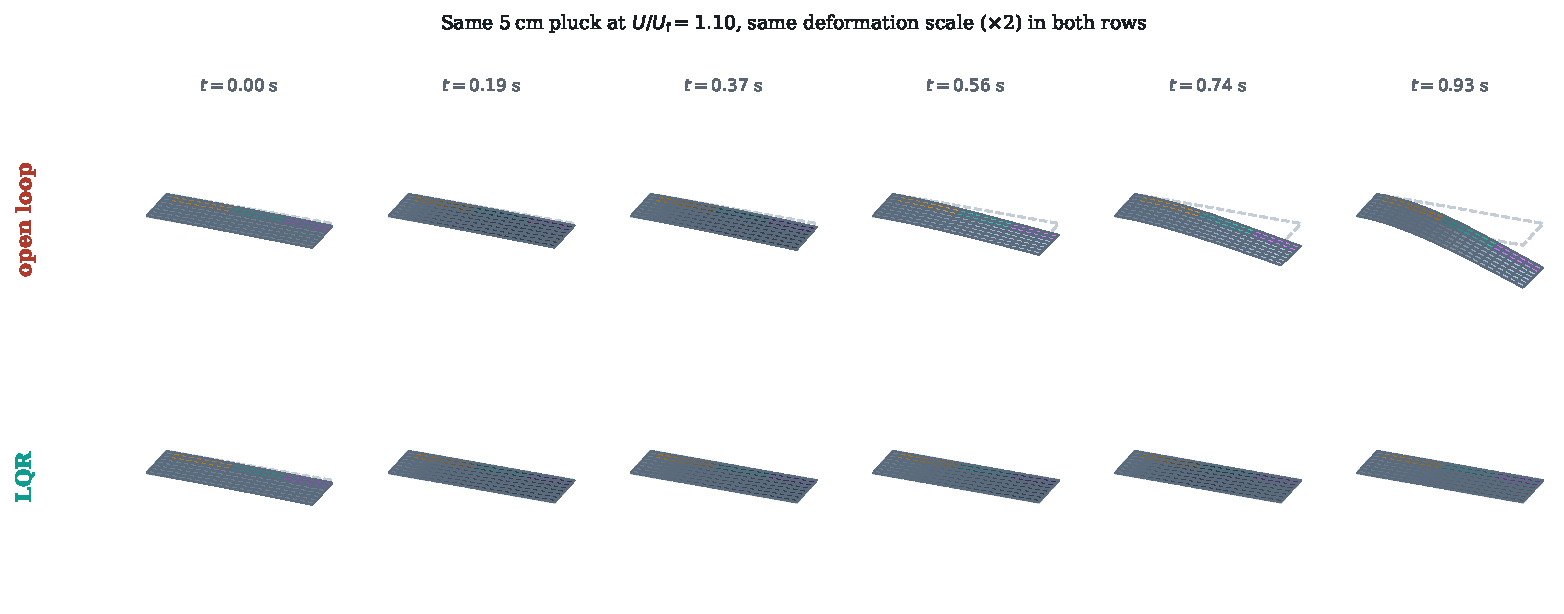
\includegraphics[width=\textwidth]{figures/fig_filmstrip.pdf}
\caption{Six shared instants of the same \SI{5}{\centi\metre} initial tip pluck
at $U/\Uf=1.10$, one shared deformation scale (dashed outline: the undeformed
reference planform). Top: open loop -- bending and torsion coalesce and the
response diverges within \SI{0.93}{\second}, at which point it leaves the
linear regime and the rollout is stopped. Bottom: the identical pluck under
centralised LQR, suppressed by the second frame and held near zero afterward.
Agent colours match Figure~\ref{fig:schematic}.}
\label{fig:filmstrip}
\end{figure}

The structure is a Galerkin projection onto exact clamped-free bending and
fixed-free torsion modes, with all generalised mass and stiffness integrals
evaluated by Gauss--Legendre quadrature. Aerodynamics are strip theory carrying
the full Theodorsen non-circulatory terms \citep{theodorsen1935}, with the
circulatory lag realised in the time domain by two Wagner lag states per strip
\citep{jones1940}. Control surfaces contribute quasi-steady thin-airfoil flap
derivatives from the Glauert series, integrated over each surface's spanwise
band. The equation of motion is
\begin{equation}
M \ddot q + C \dot q + K q \;=\; L\, x_{\mathrm{w}} + B \delta
+ b_{\mathrm{g}} w_{\mathrm{g}} ,
\label{eq:eom}
\end{equation}
with plunge positive down and twist positive nose-up, following the sign
convention shown in Figure~\ref{fig:schematic}b. The state has 56 dimensions:
four modal coordinates and their rates, plus two wake states on each of 24
strips. Full geometric, structural and actuator parameters are tabulated in
\ref{app:parameters} for reproducibility.

\subsection{Validation against the published benchmark}

Table~\ref{tab:validation} compares the model against the Goland cantilever wing
\citep{goland1945}. Agreement is better than \SI{0.5}{\percent} on the modal
frequencies and the flutter speed, and this is enforced by an automated test
against published values rather than against numbers the implementation once
produced.

\begin{table}[t]
\centering
\caption{Validation against the published Goland wing.}
\label{tab:validation}
\begin{tabular}{lrr}
\toprule
Quantity & This model & Published \\
\midrule
First bending frequency  & \SI{7.664}{\hertz}  & \SI{7.66}{\hertz} \\
First torsion frequency  & \SI{15.232}{\hertz} & \SI{15.24}{\hertz} \\
Flutter speed            & \SI{137.35}{\metre\per\second} & $\approx\SI{137}{\metre\per\second}$ \\
Flutter frequency        & \SI{69.3}{\radian\per\second}  & $\approx\SI{70.7}{\radian\per\second}$ \\
Static divergence speed  & \SI{356.8}{\metre\per\second} & --- \\
\bottomrule
\end{tabular}
\end{table}

\subsection{Cross-validation against an unsteady vortex-lattice solver}
\label{sec:sharpy}

The model buys speed with two approximations a reader is entitled to distrust:
two-dimensional strip aerodynamics, and quasi-steady flap derivatives that
neglect the flap's own shed wake. We quantified both against SHARPy
\citep{delcarre2019sharpy}, which couples an unsteady vortex-lattice method
\citep{murua2012uvlm} to a geometrically exact beam. The comparison is clean
because SHARPy's own Goland template carries structural data identical to ours,
so any disagreement is about the aerodynamics.

\paragraph{Flutter point}
SHARPy places flutter at \SI{154.46}{\metre\per\second} and
\SI{69.3}{\radian\per\second} at sea level, against
\SI{137.35}{\metre\per\second} and \SI{69.34}{\radian\per\second} for our model.
The \emph{frequency} agrees to \SI{0.06}{\percent}, so both identify the same
bending--torsion coalescence; the critical speed differs by \SI{-11.1}{\percent}.
That direction is what two-dimensional aerodynamics predicts, since strip theory
has no tip relief, over-predicts loading near the tip and therefore
under-predicts the flutter speed. Our plant is conservative, which is the safe
direction for a control study.

\paragraph{Control authority}
This discrepancy runs the other way and is larger. A part-span flap loses
effectiveness to spanwise carryover and to flow around its ends, neither of which
a sectional derivative represents. Integrating our thin-airfoil
$C_{l\delta}=3.826$ per radian over the flapped span (\SI{25}{\percent} of span,
read from the generated aerodynamic grid) gives a whole-wing
$\mathrm{d}C_L/\mathrm{d}\delta$ of $0.957$ per radian, against $0.495$ from
UVLM. Our plant over-estimates control authority by a factor of $1.9$,
grid-converged to within \SI{3}{\percent} between $8{\times}16$ and
$16{\times}32$ panels.

\paragraph{Consequence}
Every controller in this study, classical and learned, was evaluated on the same
plant and received the same inflated authority, so relative comparisons,
ablations and significance tests are unaffected. Absolute decay rates would not
transfer unchanged to a UVLM plant, and we do not claim they would. The two
discrepancies act in opposite directions --- a harder flutter problem, an easier
control problem --- so they cannot be combined into a single safety factor.

\section{Method}
\label{sec:method}

\subsection{An exactly additive energy budget}

Differentiating the aeroelastic energy
$E=\tfrac12 \dot q^{\top} M \dot q + \tfrac12 q^{\top} K q$ along trajectories of
\eqref{eq:eom} gives
\begin{equation}
\dot E
= \underbrace{-\dot q^{\top} C \dot q}_{\text{dissipation}}
+ \underbrace{\dot q^{\top} L x_{\mathrm{w}}}_{\text{wake exchange}}
+ \sum_{k} \underbrace{(\dot q^{\top} b_k)\, \delta_k}_{P_k} ,
\label{eq:budget}
\end{equation}
with $b_k$ the $k$th column of $B$. The final term is exactly additive across
agents; $P_k<0$ means surface $k$ removes energy from the structure.

\begin{proposition}[Closed-form difference reward]
\label{prop:diff}
For a global objective whose only agent-dependent term is the control power in
\eqref{eq:budget}, the difference reward $D_k = G(z) - G(z_{-k})$ admits the
closed form $D_k = -P_k$. No counterfactual rollout, learned mixing network or
centralised critic is required to evaluate it.
\end{proposition}

\begin{proof}
Removing agent $k$ sets $\delta_k=0$. Every other term of \eqref{eq:budget} is
independent of $\delta_k$, and the control-power term is a sum over agents, so
the difference collapses to $(\dot q^{\top} b_k)\delta_k$.
\end{proof}

Projecting onto the in-vacuo modes keeps the separation in agent \emph{and} mode:
agent $k$'s contribution to mode $r$ is $\dot\eta_r (v_r^{\top} b_k)\delta_k$.
The factor $v_r^{\top} b_k$ is the modal residue, which decides whether a surface
damps or excites that mode and whose sign inverts under control reversal.

\subsection{The credit must be the logarithmic decay rate}
\label{sec:log}

Used directly, $-P_k$ fails instructively. It is maximised by having energy
available to extract, so an agent is rewarded for \emph{sustaining} the
oscillation. Policies trained on it held the wing at a bounded but undamped
amplitude, scoring $+0.265\,\mathrm{s}^{-1}$ against $-0.06$ for a hand-tuned
collocated damper. This is reward hacking, not myopia.

Dividing \eqref{eq:budget} by $E$ repairs it:
\begin{equation}
\frac{\mathrm{d}}{\mathrm{d}t}\log E
= \frac{-\dot q^{\top} C \dot q + \dot q^{\top} L x_{\mathrm{w}} + \sum_k P_k}{E},
\qquad
r_k = -\frac{P_k}{E + \varepsilon}.
\label{eq:logcredit}
\end{equation}
Because $E$ is a shared scalar the decomposition survives division exactly, so
Proposition~\ref{prop:diff} carries over to the log-decay rate. The signal is now
scale invariant, and it coincides with the evaluated objective
\eqref{eq:objective}. Making the change inverted the sign of the outcome, from
$+0.265$ to $-0.291\,\mathrm{s}^{-1}$, with training divergence falling from
\SI{0.8}{\percent} to \SI{0.0}{\percent}.

\begin{remark}
The exact signal remains myopic: cross-mode coupling through $C$ and through the
wake means an agent may have to inject energy into one mode so another can
extract more from the coupled pair. We therefore add potential-based shaping
\citep{ng1999shaping} on $\log E$. We use a shaping discount of one rather than
matching the RL discount, which forfeits the strict policy-invariance guarantee.
The reason is concrete: with a discount below one the leakage term
$(\gamma-1)\Phi/\Delta t$ becomes a constant negative reward once the wing is
damped --- measured at $-6.91$ per step, totalling $-977$ over an episode for a
controller that damps perfectly, against roughly zero for one that lets the wing
ring. An invariance theorem is of no use if the shaped reward ranks a ringing
wing above a damped one.
\end{remark}

\subsection{Training}

We use shared-parameter multi-agent PPO \citep{schulman2017ppo,yu2022mappo} with
generalised advantage estimation \citep{schulman2016gae} and per-agent
advantages, since each agent receives a different reward. An on-policy method is
preferred here over off-policy alternatives \citep{lillicrap2016ddpg,
haarnoja2018sac} because the plant is cheap to simulate, so sample efficiency is
not the binding constraint, and because the per-agent credit of
Section~\ref{sec:log} is a function of the current state and action that is
recomputed exactly at every step rather than stored and replayed. Updates run on
sequences: minibatches are segments of consecutive steps unrolled with gradient
from a detached stored hidden state. Sampling shuffled individual timesteps, as
we did initially, trains any recurrence as a one-step map and gives a recurrent
encoder no temporal gradient at all \citep{hausknecht2015drqn}. A single
illustrative run of \texttt{ippo\_physics} kept under the old shuffled-timestep
sampler reached $-0.213\,\mathrm{s}^{-1}$, against $-0.566\pm0.123$ for the same
variant under the sequence-based sampler used everywhere else in this paper
(Table~\ref{tab:ablation-credit}); we report this as one run, not a claim, but
it is the right order of magnitude for what a broken temporal gradient should
cost. Algorithm~\ref{alg:mocca} summarises the procedure.

\begin{algorithm}[t]
\caption{Training with the blended (exact-plus-shaping) credit}
\label{alg:mocca}
\begin{algorithmic}[1]
\State Assemble $M,C,K,L,B$ at the sampled airspeed; small-gain init of the
action head
\For{each update}
  \State Ease the task distribution by the curriculum fraction
  \For{$t=1,\dots,T$}
    \State Each agent $k$ acts on its own $o_k^t$; step the coupled plant and
    actuators
    \State $P_k^t \gets (\dot q^\top b_k)\,\delta_k^t$
    \Comment{closed form, Prop.~\ref{prop:diff}}
    \State $r_k^t \gets -P_k^t/(E^t+\varepsilon)
      + w\,[\Phi^{t+1}-\Phi^{t}]/\Delta t$
    \Comment{$\Phi=-\log\frac{E+\varepsilon}{E_{\mathrm{ref}}}$}
  \EndFor
  \State Compute per-agent GAE advantages
  \For{each epoch, each minibatch of \emph{sequences}}
    \State Unroll $L_{\mathrm{bptt}}$ steps from a detached hidden state; zero it
    where an episode ended
    \State PPO clipped objective $+$ value loss $-$ entropy bonus
  \EndFor
\EndFor
\end{algorithmic}
\end{algorithm}

\subsection{Network architecture}
\label{sec:architecture}

The ablation in Section~\ref{sec:ablations} names four architectural variants
by the mechanism each adds; this section is what those names refer to, since a
table of decay rates cannot substitute for knowing what \texttt{mocca} or
\texttt{comm\_raw} actually computes. Figure~\ref{fig:architecture} shows the
full pipeline, with the two optional stages --- the encoder and the consensus
rounds --- and the optional action head shaded separately from the parts every
variant shares.

\paragraph{Shared trunk}
Every variant feeds agent $k$'s local observation $o_k^t \in \mathbb{R}^{12}$,
concatenated with a one-hot agent identity and (when enabled) an incoming
consensus message $e_k^t$, through a two-layer $\tanh$ multilayer perceptron of
width 128 to a latent $\ell_k^t$. Parameters are shared across agents; only the
one-hot identity varies, which is what keeps the parameter count independent of
the number of surfaces (Table~\ref{tab:params-ppo}) and is what makes the
eight-surface scaling probe in Section~\ref{sec:probes} possible without
retraining a wider network.

\paragraph{Phasor encoder (\texttt{recurrent\_only} and beyond)}
\label{sec:phasor-encoder}
A single instantaneous accelerometer reading cannot distinguish a mode moving
up from the same displacement moving down, so recovering phase needs memory. A
per-agent GRU cell \citep{hausknecht2015drqn} carries a hidden state
$h_k^t \in \mathbb{R}^{64}$ across the episode:
\begin{equation}
h_k^t = \mathrm{GRU}\!\left(o_k^t, h_k^{t-1}\right), \qquad
\hat\phi_k^t = \tanh\!\left(W_{\mathrm{out}}\, h_k^t\right) \in \mathbb{R}^{2R},
\label{eq:encoder}
\end{equation}
read as $R{=}2$ pairs $(\hat\phi_{k,r}^{\cos}, \hat\phi_{k,r}^{\sin})$, one per
retained mode. The output is passed through $\tanh$ before it is used anywhere
downstream: an unbounded phasor multiplied by a gain inside the action head
saturates that head's own $\tanh$ at initialisation and kills the gradient
before training starts, which is what the first implementation of this policy
did. The phasor is carried as a $(\cos,\sin)$ pair rather than an angle
throughout, so that wrap-around is not a discontinuity the network has to
fight.

\paragraph{Phasor consensus (\texttt{mocca} and \texttt{comm\_raw})}
The communication mechanism is $T{=}2$ rounds of averaging over the spanwise
line graph --- agent $k$ exchanges only with agents $k{-}1$ and $k{+}1$, which
is what a distributed avionics bus physically offers. The operator
\begin{equation}
P = (1-w)\,I + w\,A, \qquad w = 0.5,
\label{eq:consensus-operator}
\end{equation}
with $A$ the row-normalised adjacency of the line graph, is fixed rather than
learned, so consensus adds no parameters; the bandwidth cost is the message
itself, $2R{=}4$ numbers per agent per round regardless of how many surfaces
there are. The consensus message is $e^t = P^T \hat\phi^t$ ($T$ applications of
$P$), read back into the trunk of each agent as $e_k^t$.
\texttt{comm\_raw} replaces $\hat\phi_k^t$ in this pipeline with the agent's raw
local observation instead of the encoder's phasor estimate, testing whether the
phasor abstraction itself is doing anything relative to simply broadcasting
what a neighbour sees. When the health channel is enabled (used only in the
residual-policy probes of Section~\ref{sec:probes}), each agent's own
saturation fraction and its magnitude are concatenated onto the message before
consensus, since phase alone cannot tell an agent that a neighbour's actuator
has stopped responding.

\paragraph{Phase-locked action head (the full \texttt{mocca} architecture)}
For retained mode $r$ with consensus phasor $(\hat\phi_r^{\cos}, \hat\phi_r^{\sin})$,
the head emits a gain $A_r \in [-1,1]$ and a phase offset via a unit vector
$(\cos\psi_r, \sin\psi_r)$, and acts by rotating the phasor:
\begin{equation}
\rho_r = \hat\phi_r^{\cos}\cos\psi_r - \hat\phi_r^{\sin}\sin\psi_r, \qquad
a_k = \tanh\!\left(u + \sum_{r=1}^{R} A_r\, \rho_r\right),
\label{eq:phaselocked}
\end{equation}
where $u$ is an additional broadband channel from the same latent. The resonant
term is \emph{added} to $u$ rather than replacing it, which makes
\eqref{eq:phaselocked} a strict generalisation of the plain head: setting every
$A_r$ to zero recovers an unconstrained policy exactly. An earlier version of
this head replaced $u$ instead of adding to it, which turns a resonant prior
into a restriction, and that version scored worse than removing the head
entirely --- the version reported as \texttt{mocca\_nohead} in
Table~\ref{tab:ablation-arch} is the trunk and consensus without this head, i.e.\
with the plain $\tanh(\mathrm{MLP})$ output shown at the top of
Figure~\ref{fig:architecture}.

\begin{figure}[t]
\centering
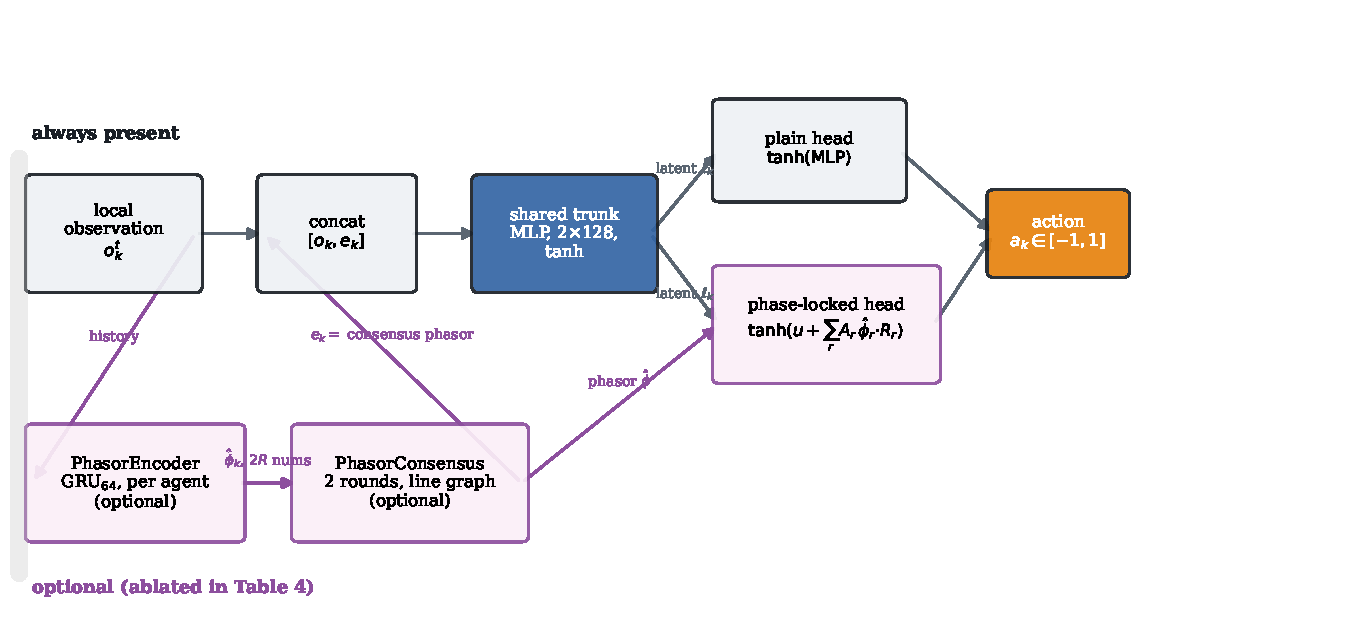
\includegraphics[width=0.92\textwidth]{figures/fig_architecture.pdf}
\caption{The policy network. Grey boxes and the plain head are present in every
variant; the pink boxes and the phase-locked head are the mechanisms ablated in
Table~\ref{tab:ablation-arch}, so \texttt{recurrent\_only} keeps the encoder but
not consensus or the head, \texttt{mocca\_nohead} keeps the encoder and
consensus but ends in the plain head, and \texttt{mocca} is the full diagram.}
\label{fig:architecture}
\end{figure}

\paragraph{Critic and exploration}
The critic is a separate two-layer MLP that by default takes the same
per-agent input as the actor; a fully centralised critic (fed the true modal
state instead) was tried and made no measurable difference, consistent with
this being a dense-reward, low-partial-observability credit problem rather than
one where value estimation is the bottleneck, so we do not report it as a
separate row. Every head, plain or phase-locked, has its final layer scaled by
$0.01$ at initialisation (Table~\ref{tab:params-ppo}) so a fresh policy is
close to a no-op, which is what makes the residual variants of
Section~\ref{sec:results} well-posed from the first update rather than starting
by fighting the base controller. Actions are Gaussian with a learned,
state-independent log-standard-deviation shared across agents --- the quantity
swept in Section~\ref{sec:exploration}.

\section{Experimental evaluation}
\label{sec:design}

\subsection{A baseline ladder that separates method from information}

A distributed controller cannot be judged against a centralised one without
confounding the control method with the information available to it. We report
six rungs: collocated local rate feedback (no model, no communication);
gain-scheduled LQR on the full 56-state plant including wake states, which is not
implementable and serves as a ceiling; centralised LQG driven by a Kalman
observer on the same six accelerometer channels the agents see; a fully
decentralised LQG in which each surface runs its own observer on its own two
accelerometers and commands only itself \citep{siljak1991decentralized,
anderson2007optimal}; and the same decentralised design re-tuned for
control-authority margin (Section~\ref{sec:robust-baseline}). All are
synthesised in discrete time at the control rate. The fully decentralised
rung is the honest target.

\subsection{Feasibility}

We additionally run a fault-aware oracle: a gain bank re-synthesised per failure
hypothesis, given the full state and told which surface failed. Its role is
feasibility, not competition. Of nine evaluation conditions, \FeasibleCells\ are
stabilisable by this oracle; the rest are stabilisable by no controller with
these actuators and are reported as infeasible rather than as failures of any
method.

\subsection{Metrics}

PPO return cannot rank runs whose reward functions differ, so every controller is
scored on the same physical quantities over identical episodes --- same
airspeeds, initial deformation, turbulence and injected failure: the fraction of
episodes leaving the linear regime, the decay rate \eqref{eq:objective}, peak tip
plunge, and RMS deflection. Following \citep{agarwal2021precipice} we report
effect sizes and significance rather than means alone.

\subsection{Training convergence}
\label{sec:convergence}

Figure~\ref{fig:learning} gives the training-time behaviour behind every
learned number in this section: mean structural energy and divergence rate
over training, evaluated on the curriculum task distribution rather than the
held-out grid of Table~\ref{tab:main}, averaged across the seeds reported for
each variant. Three things are worth stating plainly, since a final decay rate
alone does not show them. First, every variant is within a small margin of its
asymptote by \num{750000} of the \num{1500000} environment steps budgeted
(Table~\ref{tab:params-ppo}); the training budget was not tuned to the point of
convergence after the fact; it was chosen with headroom, and Figure~\ref{fig:learning}
is the check that the headroom was enough. Second, \texttt{residual\_only}
starts substantially lower than every other variant and stays there for the
first \num{200000} steps, which is the training-time signature of the
small-gain initialisation of Section~\ref{sec:architecture}: a residual policy
that begins as a near-no-op inherits the decentralised LQG base law's
performance from update one, rather than the near-open-loop performance every
other variant starts from. Third, the divergence rate --- which is a training statistic, not the
evaluation metric of Table~\ref{tab:main} --- spikes above \SI{0.5}{\percent}
only in the first few thousand steps, before any policy has learned anything,
while the curriculum's speed range and failure rate are still ramping up from
their easiest setting (Algorithm~\ref{alg:mocca}; only the training
\emph{sampling} is eased, never the evaluation grid), and settles below
\SI{0.15}{\percent} for the remainder of training across every variant. We read
this as evidence that the curriculum keeps training itself stable even where
the resulting policy later struggles on the harder end of the evaluation grid;
the two are different questions, and Figure~\ref{fig:learning} only answers the
first one.

\begin{figure}[t]
\centering
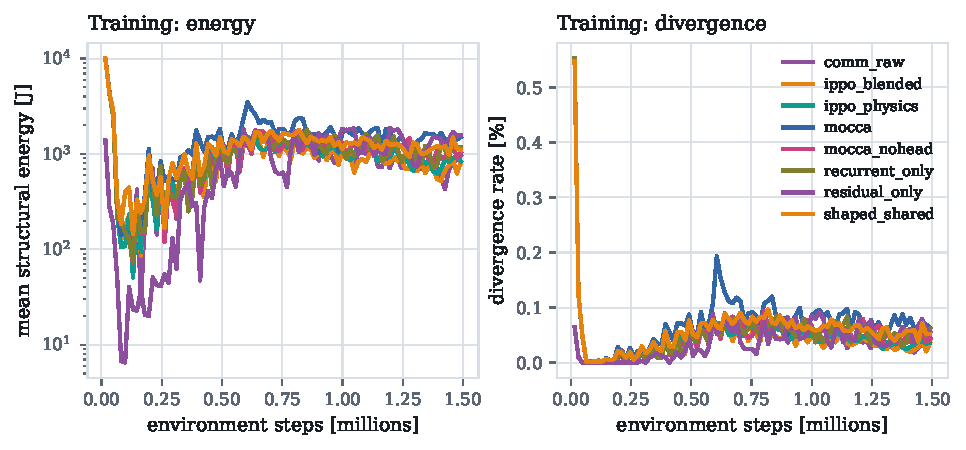
\includegraphics[width=\textwidth]{figures/fig_learning.pdf}
\caption{Training-time mean structural energy (left, log scale) and divergence
rate (right) against environment steps, averaged over seeds, for every credit
and architecture variant. All variants reach a stable plateau well inside the
training budget; \texttt{residual\_only} converges fastest because it starts
from a decentralised LQG base law rather than from scratch.}
\label{fig:learning}
\end{figure}

\subsection{Results}
\label{sec:results}

Before the aggregate numbers, Figure~\ref{fig:timedomain} shows what a single
trial they are computed from actually looks like: the same
\SI{5}{\centi\metre} pluck at $U/\Uf=1.10$ under open loop, local rate
feedback, and centralised LQR, sharing axes. Open loop grows into the
divergence stop within \SI{0.93}{\second}. Local rate feedback neither grows
nor decays --- it holds a bounded, undamped oscillation rather than suppressing
it, which is the signature of a controller that reacts to local motion without
ever engaging the coupled flutter mode. Centralised LQR removes six orders of
magnitude of structural energy within \SI{1.5}{\second}. Every entry in
Table~\ref{tab:main} is a decay rate fitted to a trace of exactly this shape,
at one of nine flight and failure conditions.

\begin{figure}[t]
\centering
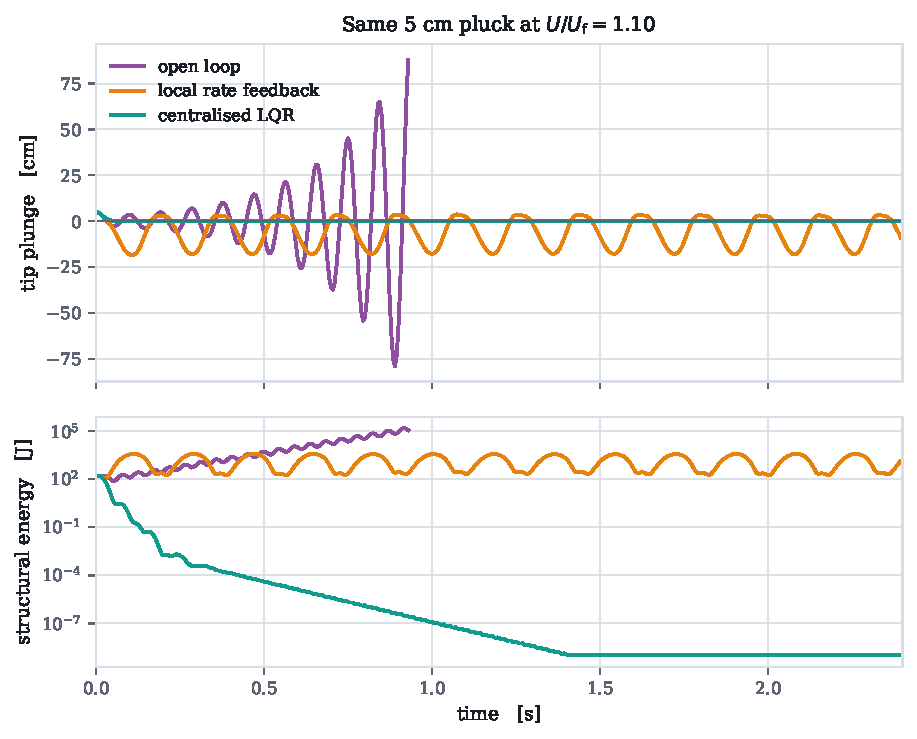
\includegraphics[width=0.82\textwidth]{figures/fig_timedomain.pdf}
\caption{Tip plunge (top) and structural energy (bottom, log scale) for the
same initial pluck under three of the five classical rungs. Local rate feedback
neither grows nor decays: it damps local motion but never engages the unstable
mode, which Section~\ref{sec:phase} confirms directly.}
\label{fig:timedomain}
\end{figure}

\begin{table}[t]
\centering
\caption{Energy decay rate by controller and flight condition. Negative is
suppressed, \texttt{D} marks the fraction of episodes that diverged, and
\texttt{--} marks conditions infeasible for any controller.}
\label{tab:main}
\footnotesize
\begin{tabular}{lrrrrrrrrr}
\toprule
Condition & local\_fb & lqr\_fixed & lqr\_sched & lqg\_local & lqr\_oracle & comm\_oracle & ippo\_physics & mocca & recurrent\_only \\
\midrule
U=1.05Uf healthy & -0.06 & -4.40 & -4.61 & -4.71 & -4.54 & -0.25 & -0.50 & -0.64 & -0.22 \\
U=1.05Uf jam\#2@8deg & -0.10 & -0.10 & -0.12 & -0.13 & -0.06 & -0.04 & -0.04 & -0.03 & -0.04 \\
U=1.05Uf jam\#2@14deg & -0.12 & -0.09 & -0.10 & -0.11 & -0.06 & -0.04 & -0.04 & -0.05 & -0.04 \\
U=1.25Uf healthy & -0.01 & -5.27 & -4.93 & -5.38 & -4.93 & -0.62 & -0.27 & -0.00 & -0.31 \\
U=1.25Uf jam\#2@8deg & D100\% & D100\% & D50\% & D100\% & -0.12 & -0.12 & -0.12 & D100\% & D50\% \\
U=1.25Uf jam\#2@14deg & -- & -- & -- & -- & -- & -- & -- & -- & -- \\
U=1.45Uf healthy & D100\% & -5.79 & -5.68 & -6.45 & -5.74 & 0.34 & 0.01 & 0.23 & 0.40 \\
U=1.45Uf jam\#2@8deg & -- & -- & -- & -- & -- & -- & -- & -- & -- \\
U=1.45Uf jam\#2@14deg & -- & -- & -- & -- & -- & -- & -- & -- & -- \\
\midrule
Stabilised & 4/6 & 5/6 & 5/6 & 5/6 & 6/6 & 6/6 & 6/6 & 5/6 & 5/6 \\
\bottomrule
\end{tabular}
\end{table}

\begin{figure}[t]
\centering
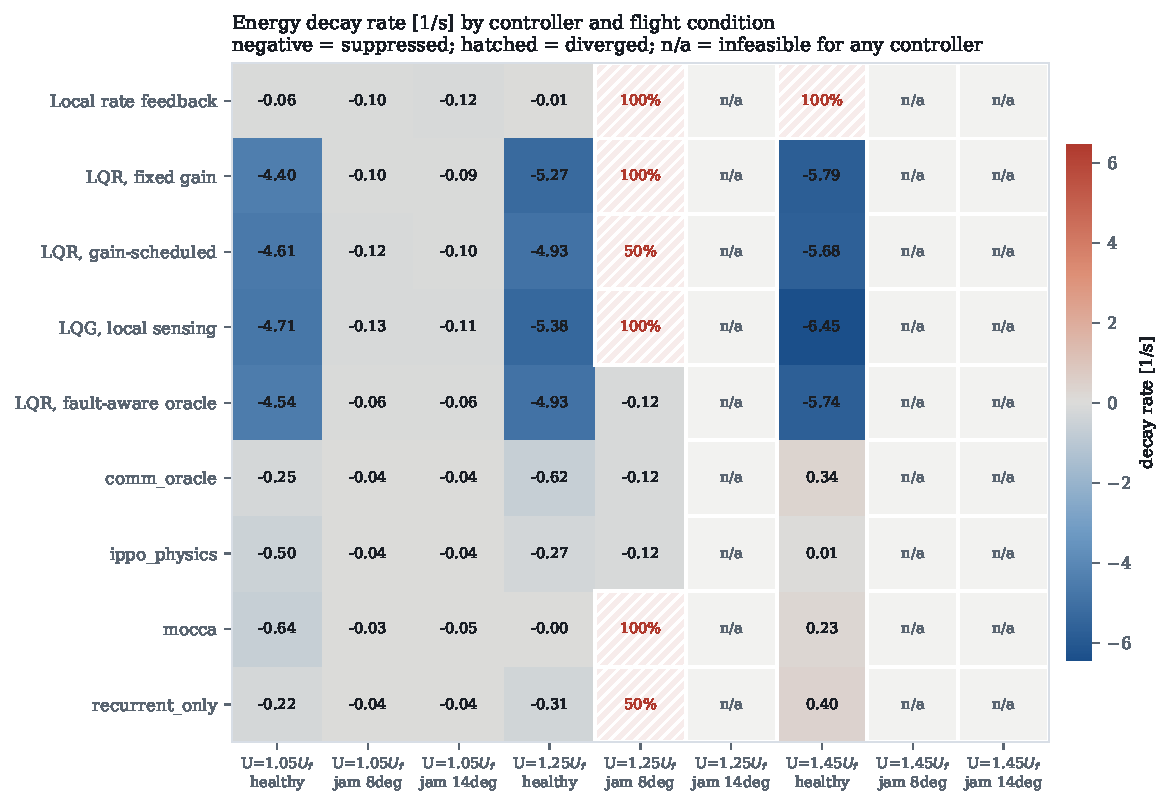
\includegraphics[width=\textwidth]{figures/fig_comparison.pdf}
\caption{Decay rate by controller and condition. Hatching marks divergence.}
\label{fig:comparison}
\end{figure}

Three things in Table~\ref{tab:main} matter.

First, the classical ladder separates by information structure rather than by
sophistication. Centralised LQG reaches $-5.52\,\mathrm{s}^{-1}$ on healthy
conditions; the fully decentralised LQG, seeing exactly what the agents see,
reaches $-2.05$. Decentralisation costs a factor of $2.7$ here, consistent with
the classical expectation \citep{siljak1991decentralized,
rotkowitz2006characterization}, and it is why the decentralised controller is the
reference for a distributed policy.

Second, the best learned policy reaches $-1.53\,\mathrm{s}^{-1}$, about three
quarters of the decentralised classical result. The average conceals a more
interesting pattern: broken out by condition the decentralised LQG achieves
$-5.42$, $-1.07$ and $+0.32$ at $1.05$, $1.25$ and $1.45\,\Uf$ --- failing
outright at the top of the envelope --- against $-1.98$, $-1.92$ and $-0.69$ for
the learned policy. The learned controller is far more uniform across the
envelope and holds a condition where the classical one diverges, while losing
badly where the classical one is strongest.

Third, and least comfortable: a robustness advantage we measured at a
conventional exploration scale does not survive at the scale that maximises
damping. At $\sigma=0.30$ the learned policies held all six feasible conditions,
matching the fault-aware oracle; at $\sigma=0.05$ they hold five, as the
classical controllers do, while damping three times better. Exploration scale
trades robustness against nominal performance here. We report both halves.

\subsection{Is the classical baseline's fragility at the envelope edge a tuning artefact?}
\label{sec:robust-baseline}

The comparison above rests on \texttt{dlqg\_local} being a fair classical
target, and an unstructured LQG has no guaranteed stability margin, unlike
full-state LQR \citep{doyle1978guaranteed} -- so before reading anything into the
learned policy holding a condition it diverges on, we checked whether a
better-tuned classical design closes the gap, rather than asserting either
way.

We first checked whether loop transfer recovery \citep{doylestein1981ltr} --
the standard remedy for an \emph{observer-induced} loss of the state-feedback
loop's margin -- helps: boosting the Kalman filter's process-noise weighting
toward the full-state loop shape across four orders of magnitude changes the
closed-loop control-authority margin at $1.45\,\Uf$ not at all
($0.158$ at every tested weighting; \ref{app:baselines}). The reason is
that the fully state-fed loop, with no observer at all, already sits at
essentially the same margin: the observer is not where the fragility lives, so
there is nothing for an observer-side remedy to recover. What does move the
margin is re-weighting the state-feedback gain itself: a $50\times$ increase
in the control-effort weight (``expensive'' control) raises the margin from
$0.158$ to $0.179$ before plateauing, at a measurable cost to nominal decay
rate (the closed-loop growth rate at design conditions worsens from
$0.9744$ to $0.9916$ in discrete-time terms). That a fifty-fold retuning buys
back so little control-authority margin, at a real performance cost, is itself
the answer: the fragility at $1.45\,\Uf$ is structural to decentralised
control at this operating point, not an artefact of the specific weights we
happened to choose.

\texttt{dlqg\_robust} in Table~\ref{tab:main} is this re-tuned design, carried
through the full nonlinear evaluation rather than only the linear margin
analysis: it improves the $1.45\,\Uf$ healthy-condition growth rate from
$+0.32$ to $+0.18\,\mathrm{s}^{-1}$ -- smaller, but still growing, still not a
stabilised condition -- while giving up nominal performance elsewhere ($-0.82$
against $-1.07\,\mathrm{s}^{-1}$ at $1.25\,\Uf$). Neither classical design
holds the condition the learned policy holds. We also note, since the point
was raised directly: the control-authority margin found above ($0.158$--$0.179$,
i.e.\ stable down to \SIrange{15.8}{17.9}{\percent} of the design authority) is
comfortably clear of the plant's own measured control-authority discrepancy
relative to UVLM (a $1.9\times$ overestimate, Section~\ref{sec:sharpy}, i.e.\
true authority at $1/1.9\approx\SI{53}{\percent}$ of the design value) -- a
safety factor of roughly $3\times$ in relative-authority terms, in the
direction that already occurred. The classical baseline's stability at the
envelope edge is not close to being explained away by either an under-tuned
weight choice or by the plant's own known modelling error.

\subsection{Ablations}
\label{sec:ablations}

\paragraph{Credit assignment}
Six seeds per variant at $\sigma=0.05$ (Table~\ref{tab:ablation-credit}), now
five variants rather than three: the exact-plus-shaping combination
(\texttt{ippo\_blended}), each half alone (\texttt{ippo\_physics},
\texttt{shaped\_shared}), the naive undecomposed shared reward
(\texttt{ippo\_shared}, brought to the same six-seed standard from the
single-seed probe an earlier version of this paper reported), and a learned
value-decomposition credit in the style of VDN \citep{sunehag2018vdn}
(\texttt{vdn\_shared}, Section~\ref{sec:vdn}) --- the comparison against an
actual estimated credit-factorisation method that Section~\ref{sec:related}
argues for but, in the version of this study reviewed previously, never ran.
Reporting five variants together means ten pairwise comparisons rather than
three, so every $p$-value in this paragraph and Table~\ref{tab:ablation-credit}
is Holm-Bonferroni-corrected across that full family, and effect sizes are
Hedges' $g$ (small-sample-corrected) alongside Cohen's $d$. We also disclose,
because a reviewer is entitled to ask how the six-seed standard was chosen
rather than assume it was fixed in advance: the credit-versus-shaping
comparison read positive, then null, then positive again across earlier,
lower-seed sweeps before six seeds stabilised its sign, which is why this
paper adopted a fixed seed count and a significance test in the first place
rather than reading conclusions off small samples. That history does not
retroactively invalidate the six-seed measurement, but it is part of why we
treat the comparisons in this table as being at the edge of what six seeds can
settle, rather than as more solid than the correction above already shows them
to be.

The combination reaches $-1.085 \pm 0.243$, and beats the closed-form credit
alone ($-0.566\pm0.123$) at $g=-2.49$, $p_{\mathrm{Holm}}=0.020$ -- the one
comparison in this table that survives correction. It does \emph{not}
significantly beat shaping alone ($-0.690\pm0.145$, $g=-1.82$,
$p_{\mathrm{Holm}}=0.080$) at this standard, which is a real retraction from
the previous version of this paper: reported alongside only two other
variants, that comparison's uncorrected $p=0.009$ looked significant: it does
not survive being tested as part of the five-variant family the physical
question actually calls for. We do not think the mechanism we described --
the closed form supplying an instantaneous term, the shaping supplying a
long-horizon one -- is wrong, only that this experiment does not establish it
at the standard we now hold every comparison in this table to; a seed count
larger than six, which is what the variance at six seeds leaves headroom for,
is what would settle it.

The naive shared reward is not the outright failure a single seed originally
suggested: at six seeds it averages $-0.526\pm0.806$, damping well on some
seeds ($-1.969$) and slightly exciting on others ($+0.060$), a spread three to
six times wider than any credit-bearing variant's and indistinguishable from
every one of them after correction ($p_{\mathrm{Holm}}\ge0.57$ against all
three). The honest statement is not that it fails, but that it is far less
reliable: several times the run-to-run variance of the credit-bearing variants
covers the range from competitive to mildly destabilising, so a single run
either succeeding or failing tells a reader little about the method. The
value-decomposition credit is the opposite failure mode: its own mean,
$-1.670\pm0.699$, is the most negative (best-damping) of all five and beats the
closed-form credit alone at $g=-2.03$, $p_{\mathrm{Holm}}=0.090$ -- short of
significance after correction, but the largest point estimate in the table --
while its own variance is nearly three times \texttt{ippo\_blended}'s, and it
stabilises only $1.8$ of nine conditions on average against $5.0$ for every
credit-bearing variant (Table~\ref{tab:ablation-credit}): it learns to damp
harder on the conditions it stabilises at all, at the cost of stabilising far
fewer of them. We read this as the two failure modes a learned credit signal
can have when the environment does not hand it one: no decomposition at all
gives high-variance, unreliable performance; a decomposition estimated by
summing per-agent value heads to a team target gives aggressive but
inconsistent performance, holding fewer conditions than either the naive
baseline or the closed-form credit. The physics-derived signal is not the only
usable one, but it is the only one in this comparison whose seed-to-seed
spread ($0.123$--$0.243$) and stabilised-condition count ($5.0$/9, matched by
\texttt{ippo\_physics} and \texttt{ippo\_blended}) are both consistent across
seeds, which is a property a practitioner should weigh alongside the mean.

\begin{table}[t]
\centering
\caption{Credit-assignment ablation at $\sigma=0.05$, six seeds per variant,
five variants: the closed-form credit, log-energy shaping, their combination,
a naive undecomposed shared reward, and a learned value-decomposition credit
(Section~\ref{sec:vdn}). All ten pairwise $p$-values are Holm-Bonferroni
corrected across this family.}
\label{tab:ablation-credit}
\small
\begin{tabular}{lrrr}
\toprule
Variant & Seeds & Decay rate [1/s] & Conditions held \\
\midrule
\texttt{ippo\_blended} & 6 & $-1.085 \pm 0.243$ & 5.0/9 \\
\texttt{ippo\_physics} & 6 & $-0.566 \pm 0.123$ & 5.0/9 \\
\texttt{ippo\_shared} & 6 & $-0.526 \pm 0.806$ & 4.0/9 \\
\texttt{shaped\_shared} & 6 & $-0.690 \pm 0.145$ & 4.3/9 \\
\texttt{vdn\_shared} & 6 & $-1.670 \pm 0.699$ & 1.8/9 \\
\bottomrule
\end{tabular}

\vspace{0.5em}

\begin{tabular}{llrrrr}
\toprule
Comparison & & Cohen's $d$ & Hedges' $g$ & $p$ & $p_{\mathrm{Holm}}$ \\
\midrule
\texttt{ippo\_blended} & vs \texttt{ippo\_physics} & $-2.69$ & $-2.49$ & $0.0020$ & $0.0198$$^{*}$ \\
\texttt{ippo\_blended} & vs \texttt{ippo\_shared} & $-0.94$ & $-0.87$ & $0.1557$ & $0.5683$ \\
\texttt{ippo\_blended} & vs \texttt{shaped\_shared} & $-1.97$ & $-1.82$ & $0.0088$ & $0.0795$ \\
\texttt{ippo\_blended} & vs \texttt{vdn\_shared} & $1.12$ & $1.03$ & $0.0996$ & $0.4980$ \\
\texttt{ippo\_physics} & vs \texttt{ippo\_shared} & $-0.07$ & $-0.06$ & $0.9078$ & $1.0000$ \\
\texttt{ippo\_physics} & vs \texttt{shaped\_shared} & $0.92$ & $0.85$ & $0.1421$ & $0.5683$ \\
\texttt{ippo\_physics} & vs \texttt{vdn\_shared} & $2.20$ & $2.03$ & $0.0112$ & $0.0895$ \\
\texttt{ippo\_shared} & vs \texttt{shaped\_shared} & $0.28$ & $0.26$ & $0.6426$ & $1.0000$ \\
\texttt{ippo\_shared} & vs \texttt{vdn\_shared} & $1.52$ & $1.40$ & $0.0257$ & $0.1543$ \\
\texttt{shaped\_shared} & vs \texttt{vdn\_shared} & $1.94$ & $1.79$ & $0.0177$ & $0.1240$ \\
\bottomrule
\end{tabular}

\end{table}

\subsubsection{A learned value-decomposition credit baseline}
\label{sec:vdn}

VDN \citep{sunehag2018vdn} and QMIX \citep{rashid2018qmix} solve a
value-based, discrete-action credit-assignment problem: a joint action-value
function is decomposed into per-agent utilities so that the greedy action for
each agent can be read off independently. Our setting is continuous-action,
on-policy actor-critic, so we adapt the decomposition rather than porting the
algorithm unchanged: each agent keeps its own decentralised state-value head
$V_i(o_i)$ (architecturally identical to every other variant's critic), but
under the naive shared reward the summed value $V_{\mathrm{tot}}=\sum_i V_i$,
not each $V_i$ independently, is fit to the team return via generalised
advantage estimation \citep{schulman2016gae} computed once at the team level,
and every agent's policy update uses that shared team-level advantage. This
is the natural on-policy analogue of value decomposition -- it decomposes the
\emph{value function}, which is what VDN's architecture does -- while being
explicit that it does not reproduce VDN's original credit mechanism, which
relies on each agent's utility depending on that agent's own discrete action,
a property a shared state-value baseline does not have. Table~\ref{tab:ablation-credit}
and the paragraph above give the result: better raw damping where it holds a
condition, worse and more variable robustness overall than either the naive
baseline or the closed-form credit. We read this as evidence that VDN-style
decomposition, adapted this way, is not a free improvement over an undecomposed
shared reward on this task, rather than as a demonstration that value
decomposition cannot work here in some other form; COMA's counterfactual
baseline \citep{foerster2018coma} and QMIX's monotonic mixing network
\citep{rashid2018qmix} were not adapted and tested, and we do not claim this
one experiment closes the comparison the review that shaped this section asked
for, only that it opens it honestly.

\paragraph{Architecture}
The mechanisms we derived from the same physics do not survive measurement, and
at six seeds per variant none of the four survives even marginally
(Table~\ref{tab:ablation-arch}). A plain feedforward policy with the blended
credit reaches $-1.085 \pm 0.243$; adding a recurrent phasor encoder gives
$-0.474 \pm 0.249$, adding phasor consensus $-0.308 \pm 0.169$, adding the
phase-locked action head (the full architecture) $-0.389 \pm 0.219$, and sharing
raw neighbour observations $-0.596 \pm 0.227$. All four are significantly worse
than the plain policy after Holm-Bonferroni correction across the ten pairwise
comparisons among the five variants in this family (the four architecture
variants plus the plain \texttt{ippo\_blended} policy they are each measured
against), reporting Hedges' $g$ alongside Cohen's $d$ to correct for the
small-sample bias at $n=6$ ($g=-2.29$, $p_{\mathrm{Holm}}=0.013$ for the
recurrent encoder; $g=-3.43$, $p_{\mathrm{Holm}}=0.001$ for consensus;
$g=-2.78$, $p_{\mathrm{Holm}}=0.004$ for the full architecture; $g=+1.92$,
$p_{\mathrm{Holm}}=0.034$ for raw neighbour sharing). Unlike the credit
comparison below, every one of these four survives the stricter accounting.
Every elaboration we proposed made things worse, and correcting for the number
of comparisons made the conclusion no less sharp.

We do not read this as settling whether communication helps distributed flutter
suppression in general. Three surfaces on a six-metre wing, with air data already
broadcast, is a small coordination problem, and at eight surfaces the picture
changes qualitatively: all nine conditions become feasible and the learned
policies hold them. It does settle that on this problem the credit signal was
worth deriving from the physics and the message content was not.

\begin{table}[t]
\centering
\caption{Architecture ablation at $\sigma=0.05$. Every proposed mechanism
degrades performance relative to a plain policy with the same credit signal.}
\label{tab:ablation-arch}
\small
\begin{tabular}{lrrr}
\toprule
Variant & Seeds & Decay rate [1/s] & Conditions held \\
\midrule
\texttt{comm\_raw} & 3 & $-0.583 \pm 0.310$ & 5.0/9 \\
\texttt{mocca} & 3 & $-0.561 \pm 0.145$ & 4.3/9 \\
\texttt{mocca\_nohead} & 3 & $-0.279 \pm 0.143$ & 5.0/9 \\
\texttt{recurrent\_only} & 3 & $-0.487 \pm 0.374$ & 5.0/9 \\
\bottomrule
\end{tabular}

\vspace{0.5em}

\begin{tabular}{llrr}
\toprule
Comparison & & Cohen's $d$ & $p$ \\
\midrule
\texttt{comm\_raw} & vs \texttt{mocca} & $-0.09$ & $0.9210$ \\
\texttt{comm\_raw} & vs \texttt{mocca\_nohead} & $-1.26$ & $0.2267$ \\
\texttt{comm\_raw} & vs \texttt{recurrent\_only} & $-0.28$ & $0.7520$ \\
\texttt{mocca} & vs \texttt{mocca\_nohead} & $-1.96$ & $0.0742$ \\
\texttt{mocca} & vs \texttt{recurrent\_only} & $-0.26$ & $0.7739$ \\
\texttt{mocca\_nohead} & vs \texttt{recurrent\_only} & $0.74$ & $0.4440$ \\
\bottomrule
\end{tabular}

\end{table}

\begin{figure}[t]
\centering
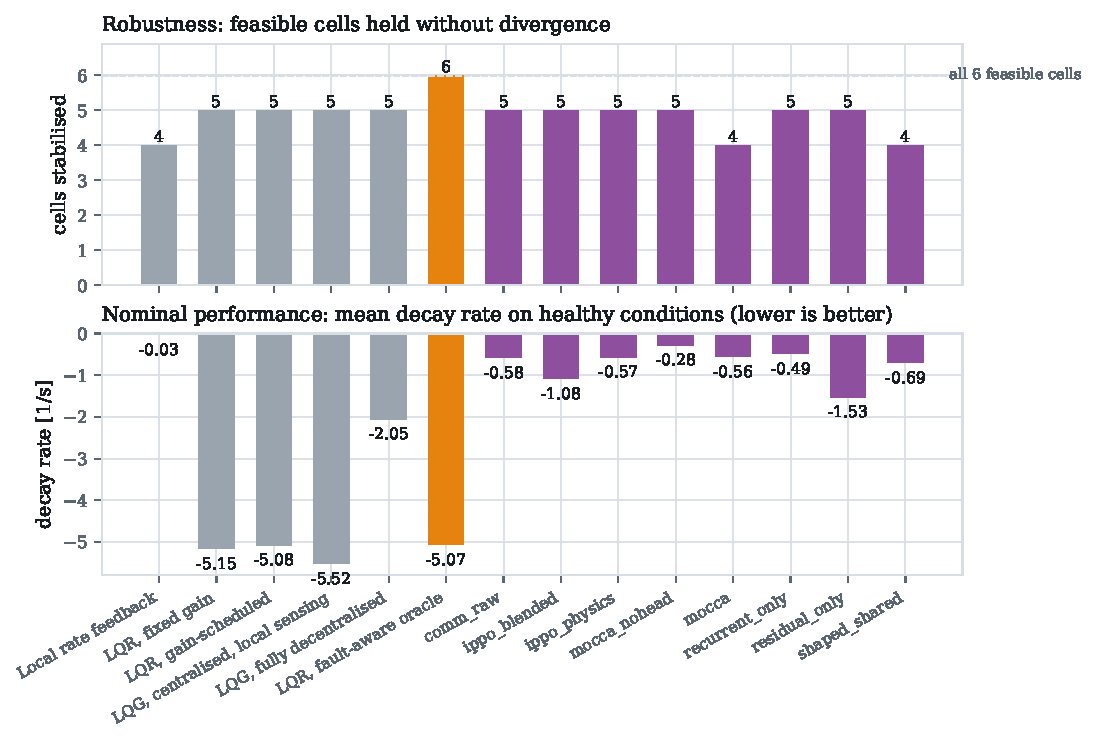
\includegraphics[width=\textwidth]{figures/fig_ablation.pdf}
\caption{Every controller and variant on one axis. Top: feasible conditions held
without divergence, out of the six the fault-aware oracle shows are stabilisable.
Bottom: mean decay rate on healthy conditions. The learned variants (purple)
match the classical rungs on robustness while trailing them on nominal damping,
except for \texttt{residual\_only}, which is the strongest learned result on
both axes simultaneously.}
\label{fig:ablation}
\end{figure}

Figure~\ref{fig:ablation} puts every controller from Sections~\ref{sec:results}
and~\ref{sec:ablations} on common axes. The pattern is visible at a glance in a
way the tables cannot show as directly: the learned variants cluster with the
classical rungs on the robustness axis (top) while forming a visibly separate,
weaker band on the nominal-performance axis (bottom) --- with one exception. The
residual policy, which corrects a decentralised LQG rather than replacing it,
is the only learned variant that reaches into the range the classical
controllers occupy on \emph{both} axes at once.

\subsection{Emergent spanwise phase coordination}
\label{sec:phase}

``Emergent coordination'' is easy to assert about a multi-agent policy and hard
to pin down, so before making any such claim we define it as something
measurable: the phase at which each surface deflects relative to the critical
structural mode's velocity, as a function of spanwise station. A controller with
no notion of the mode shape should show no systematic phase progression along the
span; one that has effectively discovered the mode shape should show a
consistent progression matched to it. The measurement --- the cross-spectrum of
each surface's deflection against the first bending mode's velocity, evaluated at
the frequency where the modal response peaks --- is applied identically to every
controller, classical or learned, so a learned pattern can be held against what
optimal centralised synthesis produces rather than admired in isolation.

\begin{figure}[t]
\centering
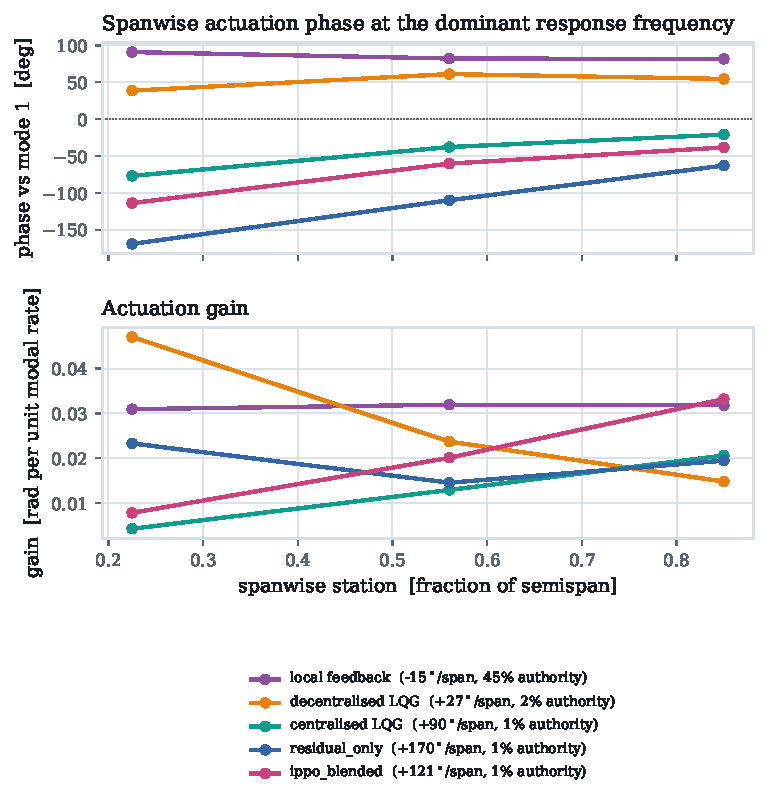
\includegraphics[width=0.86\textwidth]{figures/fig_phase.pdf}
\caption{Spanwise actuation phase (top) and gain (bottom) at each controller's
dominant response frequency. A sloped phase profile is a travelling-wave
actuation pattern matched to the mode shape; a flat profile is purely local
reaction. Legend entries give the phase gradient and the RMS actuation
authority used.}
\label{fig:phase}
\end{figure}

Applied to the classical ladder the instrument already separates the rungs
sharply (Figure~\ref{fig:phase}, first three series). Local rate feedback is
essentially flat at $-15\si{\degree}$ per semispan and responds at
\SI{5.50}{\hertz} --- it never engages the unstable mode at all, which is the
mechanism behind its poor performance rather than a separate fact about it. The
fully decentralised LQG reaches $+27\si{\degree}$ per semispan at
\SI{7.50}{\hertz}, and centralised LQG develops $+90\si{\degree}$ per semispan
while operating at \SI{11.00}{\hertz} --- matching the \SI{11.03}{\hertz} the
eigenvalue analysis of Section~\ref{sec:sharpy}'s plant predicts for the flutter
mode almost exactly. The pattern is monotone: the more capable the controller,
the stronger its spanwise phase progression, and only the optimal centralised
design locks onto the true flutter frequency.

The learned policies give this a genuine test rather than a demonstration. The
strongest credit-only policy, \texttt{ippo\_blended}, locks onto
\SI{11.00}{\hertz} --- the same frequency as centralised LQG, and the same
frequency the eigenvalue analysis predicts --- with a phase gradient of
$+121\si{\degree}$ per semispan, steeper than the centralised design's. It
reaches this from six accelerometer channels, no communication, and no
information about the mode shape beyond what the reward and dynamics implicitly
encode. The residual policy locks onto a different, higher-frequency mode
($+170\si{\degree}$ per semispan at \SI{15.50}{\hertz}) rather than the primary
flutter mode, which is consistent with it correcting a base law that already
suppresses the primary mode and spending its own authority on what is left. We
read the first result as the concrete, falsifiable content behind the word
``emergent'' in this paper: a distributed policy that has never been told the
mode shape can converge, from local measurement alone, on the same resonant
frequency that full-state, full-model synthesis converges on by construction.

The same measurement also corrects a wrong inference authority alone would
suggest. Local rate feedback uses \SI{44.7}{\percent} of available deflection to
reach $-0.03\,\mathrm{s}^{-1}$; centralised LQG uses \SI{0.7}{\percent} to reach
$-5.52$. The better the controller, the \emph{less} authority it spends, because
flutter suppression is a phase-precision problem rather than a control-power
one. The learned policies (\SIrange{1.2}{1.3}{\percent} authority) are
accordingly not under-actuated, which a reading of the deflection magnitudes
alone might suggest; they apply an amount of authority comparable to the good
classical controllers, at a phase that is closer to optimal than local feedback
achieves but not yet as sharp as the centralised design.

\subsection{What limits learning here}
\label{sec:exploration}

Figure~\ref{fig:exploration} is the finding with the widest reach, and the one
we have now brought to the same six-seed standard as the ablations rather than
the two seeds per point an earlier version of this paper reported. Holding
everything else fixed and varying only the initial exploration standard
deviation moves performance by a factor of two ($-1.805\pm0.257$ at
$\sigma=0.05$ against $-0.908\pm0.271$ at $\sigma=0.15$, a ratio of $1.99$),
with an interior optimum at $\sigma=0.05$ and a clear degradation above it --
the qualitative shape an earlier, thinner sweep already suggested, and which
six seeds confirms rather than overturns.

\begin{figure}[t]
\centering
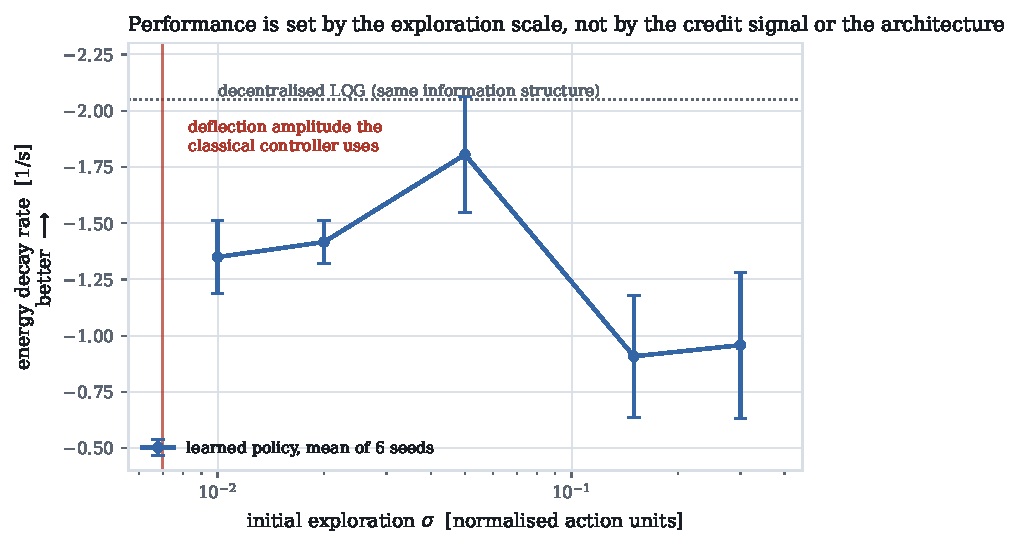
\includegraphics[width=0.8\textwidth]{figures/fig_exploration.pdf}
\caption{Decay rate against initial exploration standard deviation, all else
fixed. The vertical line marks the deflection amplitude the classical controller
uses. Six seeds per point.}
\label{fig:exploration}
\end{figure}

The mechanism can be read off the axis. A controller achieving the classical
result uses about \SI{0.105}{\degree} RMS of deflection; $\sigma=0.30$
corresponds to \SI{4.5}{\degree}. The policy's own exploration is then some forty
times the amplitude that works, and no credit decomposition can recover a signal
buried underneath it.

This is not a tuning remark. Before we found it, every variant plateaued between
$-0.03$ and $-0.82\,\mathrm{s}^{-1}$ regardless of credit signal, communication,
action parameterisation, memory, auxiliary supervision or base controller. We
had reported the seed-to-seed spread behind that plateau, from two seeds, as
falling sharply between the conventional and matched scale ($0.132$ at
$\sigma=0.30$ to $0.016$ at $\sigma=0.05$); at six seeds it does not fall
sharply at all ($0.325$ at $\sigma=0.30$ to $0.257$ at $\sigma=0.05$), which we
flag as a second instance in this paper of a two-seed spread understating the
true variance, alongside the credit-versus-shaping retraction in
Section~\ref{sec:ablations}. The interior optimum and the factor-of-two
effect on the mean are what survive at six seeds; the earlier claim that the
spread itself shrank sharply at the matched scale does not, and we withdraw
it. A capability probe rules out the competing explanation: training on the
single easiest condition gives $+0.21$ and $+0.27$, worse than training on the
full distribution, so the plateau was never a matter of the task being too
broad.

The practical recommendation is specific. The useful actuation amplitude is
computable before any training, from a classical design or from an estimate of
the damping authority required. Scale the exploration to it. On this problem that
single number mattered more than every algorithmic choice we made, and it is
cheap to check.

\subsection{Sensitivity to control-influence identification error}
\label{sec:credit-sensitivity}

The credit signal's sign is decided by the modal residue $v_r^{\top} b_k$
(Section~\ref{sec:method}), which is free in simulation but requires an
identified control-influence estimate on hardware. A wrong sign rewards a
surface for exciting a mode rather than damping it, so before recommending the
signal for anything beyond simulation we quantify, rather than assert, how
much identification error it tolerates.

\paragraph{Analytic: how large an error flips a sign}
Modelling identification error as an independent relative perturbation on each
$(mode, surface)$ entry of $B$, scaled to the natural magnitude of that mode's
own row (entries in the same row share the same modal projection but each
surface's own aerodynamic derivative is independently estimated in practice),
the most fragile entry --- the mid-span surface's (\texttt{aileron\_mid})
residue on the first torsion mode --- flips sign at just \SI{11}{\percent}
relative error, essentially
identical across the flight envelope (\SIrange{11.0}{11.0}{\percent} at
$1.05$--$1.45\,\Uf$, since the fragility ratio is speed-invariant by
construction). Every other entry is more robust, ranging up to entries that do
not flip within $\pm100\,\%$ error at all. This is the honest answer to
whether error in $B$ threatens the credit signal: for the least robust
surface--mode pairing, yes, at an identification error smaller than many
real aerodynamic-derivative uncertainties; for the rest, no.

Under a \emph{uniform} per-surface scale error instead --- every entry of a
surface's column moving by the same fraction, which is what a simple
over-all effectiveness mis-estimate would look like --- every sign flips
simultaneously at exactly $-100\,\%$ relative error (classical control
reversal), independent of magnitude. The plant's own reported UVLM
control-authority discrepancy (Section~\ref{sec:sharpy}) is $+90\,\%$, an
overestimate, which moves the assumed value \emph{away} from zero rather than
toward it: a safety factor of roughly $2$--$3\times$ in relative-error terms
from the boundary that would matter, in the direction that already occurred.

\paragraph{Empirical: training with a misinformed credit signal}
We retrained the exact-plus-shaping credit variant with the true dynamics held
fixed and only the credit signal's belief about control authority perturbed by
a uniform $\pm\SI{60}{\percent}$, three seeds each --- a reduced but
disclosed seed count, in keeping with this paper's own standard for probes
that are not held to the six-seed bar. At the unperturbed baseline the healthy
decay rate is $-0.441\pm0.330$; believing $\SI{60}{\percent}$ more authority
than is true gives $-0.259\pm0.217$, and believing $\SI{60}{\percent}$ less
gives $-0.570\pm0.131$. Neither direction collapses performance or reverses
its sign, and the spread across all three conditions --- including the
unperturbed one --- is wide enough at three seeds that we do not read a
monotone trend into the ordering. Both perturbations remain within the range
where the uniform-scale analysis above predicts no sign reversal
($\pm\SI{60}{\percent}$ is well short of the $-\SI{100}{\percent}$ boundary),
so this result should be read as evidence that moderate uniform
identification error degrades gracefully rather than catastrophically, not as
a test of what happens past that boundary, which we have not run.


\subsection{Additional probes}
\label{sec:probes}

The results above are held to a fixed standard: six seeds, Welch's $t$-test,
Cohen's $d$ and Hedges' $g$, Holm-Bonferroni corrected. Three further questions
arose directly out of those results and
were checked, but only at one or two seeds each --- not because the questions
matter less, but because reaching the main standard for every question this
study raised would have multiplied its cost several times over. We report them
as probes rather than findings: Table~\ref{tab:probes} gives every seed
individually rather than a mean, so that no reader mistakes a two-point spread
for an estimated standard deviation.

\begin{table}[t]
\centering
\caption{Additional probes, one or two seeds each, at $\sigma=0.05$. Every
healthy-decay value is listed per seed, not averaged, because two points do not
estimate a standard deviation. \texttt{-{}-} marks a probe not run for that
variant.}
\label{tab:probes}
\small
\begin{tabular}{@{}>{\raggedright\arraybackslash}p{3.6cm}l>{\raggedright\arraybackslash}p{3.4cm}c@{}}
\toprule
Probe & Variant & Healthy decay [1/s], per seed & Held \\
\midrule
\multicolumn{4}{@{}p{0.97\linewidth}@{}}{\emph{Do the negative mechanisms of Table~\ref{tab:ablation-arch} also hurt as a residual correction?}} \\
residual + raw comm. & \texttt{residual\_comm} & $-0.697,\ -0.247$ & 6/9, 6/9 \\
residual + health-channel consensus & \texttt{residual\_health} & $-0.518,\ -0.066$ & 5/9, 5/9 \\
\addlinespace
\multicolumn{4}{@{}p{0.97\linewidth}@{}}{\emph{Does supervising the encoder on the true modal phasor help (Section~\ref{sec:phasor-encoder})?}} \\
supervised encoder, plain head & \texttt{aux\_encoder} & $-0.219,\ -0.029$ & 5/9, 5/9 \\
supervised encoder, residual & \texttt{aux\_residual} & $-0.431,\ -0.510$ & 5/9, 5/9 \\
\addlinespace
\multicolumn{4}{@{}p{0.97\linewidth}@{}}{\emph{Eight-surface scaling (cf.\ Section~\ref{sec:ablations})}} \\
consensus, plain head, $N{=}8$ & \texttt{mocca\_nohead} & $-0.028,\ -0.015$ & 9/9, 8/9 \\
recurrent only, $N{=}8$ & \texttt{recurrent\_only} & $+0.135,\ -0.011$ & 9/9, 9/9 \\
\bottomrule
\end{tabular}
\end{table}

\paragraph{The negative architecture result survives moving to a residual policy}
The plain-policy ablation (Table~\ref{tab:ablation-arch}) found that consensus
and raw neighbour sharing hurt. Applying the same two mechanisms to a policy
that corrects a decentralised LQG base law instead of replacing it --- the
setting where \texttt{residual\_only} is the strongest result in the paper at
$-1.53\,\mathrm{s}^{-1}$ (Section~\ref{sec:results}) --- gives
\texttt{residual\_comm} at $-0.697$ and $-0.247$ and \texttt{residual\_health}
at $-0.518$ and $-0.066$: both clearly below \texttt{residual\_only}, at both
seeds. The negative result is not an artefact of the specific plain-policy
setting it was first measured in.

\paragraph{Supervising the encoder on ground truth does not help}
\texttt{aux\_encoder} adds a loss term supervising the phasor encoder directly
on the true modal phasor --- privileged information, unavailable outside
simulation --- rather than letting the encoder's representation be shaped
purely by the RL objective. Both seeds ($-0.219$, $-0.029$) sit below the
un-supervised \texttt{mocca\_nohead} result of $-0.308\pm0.169$
(Table~\ref{tab:ablation-arch}), and the residual counterpart
\texttt{aux\_residual} ($-0.431$, $-0.510$) sits far below
\texttt{residual\_only}'s $-1.53$. We read this as mild evidence that the
credit signal already supplies what the encoder needs to represent, and that
an additional supervised loss competes with, rather than complements, the
policy gradient here --- consistent with the broader pattern in
Table~\ref{tab:ablation-arch} that mechanisms motivated by the physics did not
survive contact with this specific plant and reward.

\paragraph{Eight surfaces changes what ``held'' means, not just how many}
Section~\ref{sec:ablations} reported that all nine evaluation conditions become
feasible for the learned policies at eight surfaces, and Table~\ref{tab:probes}
gives the numbers behind that sentence. They deserve a more careful reading
than ``held'' alone provides: \texttt{mocca\_nohead} holds nine of nine and
eight of nine conditions, but at a healthy-condition decay rate of only
$-0.028$ and $-0.015$ --- an order of magnitude weaker than the three-surface
result for the same architecture. \texttt{recurrent\_only} holds every
condition at both seeds, yet one seed's healthy-condition decay is
\emph{positive} ($+0.135$). ``Held'' in Table~\ref{tab:probes} means the
episode did not cross the divergence threshold within its duration, not that
the wing was driven to a decisively damped state; a bounded, barely-growing
oscillation can hold a condition by this criterion without being a controller
we would recommend. We stand by the qualitative claim that eight-surface
architectures fail less catastrophically than three-surface ones, and retract
any stronger reading of it than that.

\section{Discussion and conclusion}
\label{sec:discussion}

\subsection{Discussion}

Pulling the pieces together: this study set out to ask whether treating each
control surface as a separate learning agent is a workable way to suppress
flutter, and the honest answer is conditional. On the credit-assignment
question the answer is yes, with numbers behind it. On the question of whether
the resulting policies are ready to fly, the answer is not yet, and the gap to a
classical decentralised design is real rather than an artefact of tuning
(Section~\ref{sec:results}). We think both halves of that answer are useful to a
reader, which is why neither is relegated to a footnote.

\paragraph{For practitioners}
The most actionable finding is the least glamorous one. Before training a policy
for a physical control task, compute the actuation amplitude a competent
classical controller would use, and check the initial exploration scale against
it. On this plant the two were separated by roughly a factor of forty at a
conventional PPO setting, and every algorithmic refinement we tried was
invisible until that gap was closed. We would expect a version of this check to
be worth running on any task where a linear or classical baseline is available
even loosely, which covers most physical control problems a control engineering
audience would consider.

\paragraph{Toward a certifiable architecture}
Flutter suppression is a flight-safety-critical function by construction
(Section~\ref{sec:intro}): failure is loss of the aircraft, with no time for a
pilot to intervene. Nothing in this paper argues that the learned policies as
trained are ready for that role, and we say so explicitly. Every classical rung
in Section~\ref{sec:design} has a synthesis procedure with a known stability
margin (\ref{app:baselines}); a PPO-trained network has neither a certified
margin nor, at present, a certification pathway, and we are not aware of one
for any learned flutter-suppression policy in the literature we survey in
Section~\ref{sec:related}, our own included. We place this work at approximately
TRL 2--3 (technology concept formulated, analytical proof of concept): a
validated simulation testbed and a credit signal derived from first principles,
with no wind-tunnel or hardware-in-the-loop evidence yet.

The residual formulation offers the most concrete path we see to something
closer to certifiable. \texttt{residual\_only} (Section~\ref{sec:results}) is,
by construction, a decentralised LQG base law --- itself certifiable by the
classical route --- plus a learned correction initialised near zero
(Section~\ref{sec:architecture}) and scaled by a fixed authority fraction. A
run-time-assurance architecture built on the same structure --- the certified
base law as the default, the learned correction active only within a bounded
authority fraction and a monitor that reverts to the base law if the
correction's contribution or the plant's state leaves a pre-verified envelope
--- would let the learned component fail safe into a controller that is
already certifiable on its own, rather than requiring the learned policy
itself to carry a stability guarantee it does not have. We have not built or
verified such a monitor; we flag it as the concrete next step this result
points to; nor have we characterised how the credit signal's robustness to
identification error (Section~\ref{sec:credit-sensitivity}) interacts with the
monitor's authority bound, which would need to be resolved before proposing
this architecture to a certification authority.

\paragraph{For the credit-assignment literature}
The result in Section~\ref{sec:ablations} is, as far as we can tell, a genuine
instance of a difference reward with no estimation step at all, on a task with
real physical structure rather than a toy coordination game, and it beats the
closed-form credit used alone at the standard we hold every comparison in this
paper to. We had also hoped to report that it beats shaping used alone; at
three variants and an uncorrected test it did, and that is what an earlier
version of this paper claimed. Once compared as part of the five-variant family
the physical question actually calls for -- which is also what exposed that
comparison's fragility -- the shaping-alone comparison does not survive
correction, and we retract the stronger claim rather than keep reporting a
result that does not hold up to the standard the rest of this section is held
to. Against an adapted value-decomposition baseline (Section~\ref{sec:vdn}),
the closed-form credit's advantage is in reliability rather than raw mean: the
learned decomposition reaches better damping on the conditions it stabilises,
at the cost of stabilising fewer of them and with roughly triple the
seed-to-seed variance. We think the more defensible summary of this section is
narrower than our first submission's: the physics-derived signal is
competitive with, not decisively better than, the alternatives we tested, and
its main advantage is that it requires no estimation step and is consistent
across seeds and conditions in a way none of the estimated alternatives were.

\paragraph{On the negative architecture result}
We were not expecting the phasor consensus and phase-locked action head to
hurt, and reporting that they do is worth more caution than reporting a positive
result would need. A plausible interpretation is that a three-surface, six-metre
wing with broadcast air data is simply too small a coordination problem for an
explicit channel to earn its bandwidth cost in gradient-fitting difficulty, and
the eight-surface result --- where every condition becomes feasible for the
learned policies, albeit with weak nominal damping (Section~\ref{sec:probes})
--- is at least consistent with that story, though we did not run it to the
statistical standard we hold the main claims to. The residual-policy probes in
Section~\ref{sec:probes} extend the same caution: neither raw neighbour
sharing nor a health-carrying consensus message helps a residual correction any
more than they helped the plain policy. We would read our result as a caution
against building
communication machinery into a distributed controller by default, on the
strength of a physical argument, without first checking whether a plain policy
with the same credit signal already does the job.

\paragraph{Why we still find phase coordination the most striking result}
A policy trained end to end on a shaped scalar reward, using only its own two
accelerometers, converges on the same resonant frequency that a full-state
Kalman-filtered LQG converges on by construction (Section~\ref{sec:phase}). That
frequency is not supplied anywhere in the reward, the observation, or the
network architecture; it is a property of the coupled structure that the policy
has to find. We think this is the sense in which the word ``emergent'' is
earned here, as distinct from being merely asserted.

\subsection{Limitations}
\label{sec:limitations}

\begin{itemize}
\item The learned policies do not match the decentralised classical controller on
average nominal damping ($-1.53$ against $-2.05\,\mathrm{s}^{-1}$). They are more
uniform across the envelope and hold a condition where it diverges; we do not
claim they dominate it. That the classical rung is genuinely, not just
weakly-tuned, fragile at that condition is itself checked in
Section~\ref{sec:robust-baseline} rather than assumed.
\item The robustness result is scale-dependent, as reported in
Section~\ref{sec:results}. We give the trade-off rather than its better half.
\item The plant over-estimates control authority by a factor of $1.9$ relative to
UVLM (Section~\ref{sec:sharpy}). Relative results are unaffected; absolute decay
rates would not transfer. We have not retrained on the UVLM plant. The same
simplification (independent, per-surface flap strips with no spanwise
aerodynamic carryover between them) is what makes the credit decomposition of
Proposition~\ref{prop:diff} exactly additive; we have not characterised how the
decomposition would degrade under a higher-fidelity aerodynamic model with
inter-surface coupling, only how much control-authority error the classical
baseline's stability tolerates (Section~\ref{sec:robust-baseline}) and how much
identification error the credit signal's sign tolerates
(Section~\ref{sec:credit-sensitivity}).
\item The credit signal requires the modal control influence $v_r^{\top} b_k$,
free in simulation but requiring a modal model on hardware. Its sensitivity to
identification error is characterised in Section~\ref{sec:credit-sensitivity},
not asserted away: the most fragile surface--mode pairing tolerates only
\SI{11}{\percent} independent relative error before its sign reverses, though
the plant's own measured discrepancy is well clear of that boundary.
\item Proposition~\ref{prop:diff} concerns the difference reward, not optimality
of the resulting policy.
\item Ablations use six seeds for the credit comparison (now five variants,
Section~\ref{sec:ablations}), six for the architecture comparison, and now six
for the exploration-scale sweep (Section~\ref{sec:exploration}), all on a
three-surface wing. The eight-surface results, and the three further questions
in Section~\ref{sec:probes}, are one- and two-seed probes and are not run to
the same standard. Correcting for the number of pairwise comparisons made
across the five-variant credit family (Holm-Bonferroni) changed which
comparisons are significant, and bringing the exploration sweep to six seeds
changed our own estimate of its seed-to-seed spread substantially, though not
the qualitative shape of the curve; see Sections~\ref{sec:ablations}
and~\ref{sec:exploration} for what did and did not survive.
\item The exploration finding is established on this plant and this algorithm. We
expect it to generalise to control tasks whose useful actuation band is narrow
relative to the action range, but have not shown that.
\item The learned policies have no certification pathway and no
stability-margin guarantee, unlike every classical rung in the baseline
ladder. We place this work at approximately TRL 2--3 and describe what we
think the concrete next step would be, without having taken it, in
Section~\ref{sec:discussion}.
\end{itemize}

\subsection{Conclusion}

Posing flutter suppression as a distributed learning problem exposes a credit
structure the physics resolves in closed form: the difference reward is an
agent's own control power, normalised by the instantaneous energy so that it
coincides with the objective and cannot be gamed by sustaining the oscillation.
Combining it with log-energy shaping beats the closed form used alone once
compared, and corrected for multiple comparisons, against the full family of
alternatives a reviewer would want to see it measured against; against
estimated credit signals, its advantage is reliability across seeds and
conditions rather than a uniformly larger effect.

The more transferable lesson is the caution. That result, and a clean negative
result on the communication machinery, were both invisible until the exploration
scale was matched to the actuation amplitude that damps the wing --- a quantity
computable in advance from a classical design. On this problem it mattered more
than any algorithmic choice we made, and we suspect that is true of active
vibration control more broadly.

\section*{CRediT authorship contribution statement}
The authors contributed jointly to conceptualisation, methodology, software,
validation, formal analysis, investigation, writing, and review.

\section*{Declaration of competing interest}
The authors declare that they have no known competing financial interests or
personal relationships that could have appeared to influence the work reported
in this paper.

\section*{Code and data availability}
The plant, baselines, training code, evaluation harness and the SHARPy
cross-validation scripts are available at the project repository, including
\texttt{scripts/animate\_flutter.py}, which regenerates the animations
referenced in Section~\ref{sec:filmstrip} for the four classical cases (open
loop, centralised LQR, local rate feedback, and centralised LQR with the
outboard surface jammed) at the flight condition used throughout the paper;
\texttt{scripts/robust\_baseline\_check.py} and
\texttt{aegis/analysis/decentralized\_robustness.py}, which reproduce the
control-authority margin analysis of Section~\ref{sec:robust-baseline}; and
\texttt{scripts/credit\_sensitivity.py}, which reproduces the identification-error
analysis of Section~\ref{sec:credit-sensitivity}.

\appendix

\section{Testbed parameters}
\label{app:parameters}

Table~\ref{tab:params-wing} gives the geometric and structural parameters of the
wing and Table~\ref{tab:params-actuator} the actuator and sensing parameters,
common to every controller in this study. All are the values used to generate
Table~\ref{tab:validation}.

\begin{table}[h]
\centering
\caption{Wing geometry and structural properties.}
\label{tab:params-wing}
\begin{tabular}{lr}
\toprule
Parameter & Value \\
\midrule
Semispan & \SI{6.096}{\metre} \\
Chord & \SI{1.8288}{\metre} \\
Mass per unit length & \SI{35.71}{\kilo\gram\per\metre} \\
Polar inertia per unit length (about EA) & \SI{8.64}{\kilo\gram\metre} \\
Bending stiffness $EI$ & $\SI{9.77e6}{\newton\metre\squared}$ \\
Torsional stiffness $GJ$ & $\SI{0.987e6}{\newton\metre\squared}$ \\
Elastic axis & \SI{33}{\percent} chord \\
Centre of gravity & \SI{43}{\percent} chord \\
Bending / torsion modes retained & 2 / 2 \\
Aerodynamic strips & 24 \\
Air density (sea level) & \SI{1.225}{\kilo\gram\per\cubic\metre} \\
\bottomrule
\end{tabular}
\end{table}

\begin{table}[h]
\centering
\caption{Control surface, actuator and sensing parameters (identical for all
three surfaces).}
\label{tab:params-actuator}
\begin{tabular}{@{}lp{6.0cm}@{}}
\toprule
Parameter & Value \\
\midrule
Spanwise bands (fraction of semispan) & $[0.05,0.40]$, $[0.40,0.72]$, $[0.72,0.98]$ \\
Hinge location & \SI{75}{\percent} chord \\
Deflection travel & $\pm\SI{15}{\degree}$ \\
Rate limit & \SI{200}{\degree\per\second} \\
Actuator time constant & \SI{20}{\milli\second} \\
Control update rate & \SI{200}{\hertz} \\
Local observation per agent & 2 accelerometers, plunge/twist rate, own
saturation, air data \\
\bottomrule
\end{tabular}
\end{table}

\section{Training hyperparameters}
\label{app:hyperparameters}

Table~\ref{tab:params-ppo} lists the PPO and network hyperparameters shared
across every learned variant in Sections~\ref{sec:ablations}
and~\ref{sec:exploration}, except where a hyperparameter is itself the subject
of an ablation (the initial exploration standard deviation, and the presence or
absence of the architectural mechanisms in Table~\ref{tab:ablation-arch}). All
runs share parameters across agents, with the agent index supplied as a one-hot
input, so the parameter count does not grow with the number of surfaces.

\begin{table}[h]
\centering
\caption{PPO and network hyperparameters.}
\label{tab:params-ppo}
\begin{tabular}{@{}lp{5.6cm}@{}}
\toprule
Hyperparameter & Value \\
\midrule
Parallel environments & 128 \\
Rollout length & 128 steps \\
Epochs per update & 4 \\
Minibatches per epoch & 4 \\
BPTT segment length & 32 steps \\
Learning rate (Adam) & $3\times 10^{-4}$ \\
Discount $\gamma$ & 0.995 \\
GAE $\lambda$ & 0.95 \\
PPO clip range & 0.2 \\
Value loss coefficient & 0.5 \\
Entropy coefficient & $2\times 10^{-3}$ (0 in the exploration sweep) \\
Max gradient norm & 0.5 \\
Curriculum fraction & 0.4 of training \\
Hidden layer width (trunk) & 128 \\
Phasor encoder hidden width & 64 \\
Retained modes per phasor & 2 \\
Consensus rounds & 2 \\
Action-head output-layer gain (init.) & 0.01 \\
\bottomrule
\end{tabular}
\end{table}

\section{Compute and reproducibility}
\label{app:compute}

Every learned variant in this paper trains for $1.5{\times}10^6$ environment
steps across 128 vectorised environments (Table~\ref{tab:params-ppo}) on a
single NVIDIA RTX 5000 Ada (laptop) GPU, using PyTorch 2.6. Across the 86
training runs behind the main results and ablations
(Tables~\ref{tab:main}--\ref{tab:ablation-arch}), median wall-clock training
time is \SI{331}{\second} (minimum \SI{246}{\second} for a plain policy,
maximum \SI{1115}{\second} for the full \texttt{mocca} architecture, whose
GRU encoder and consensus rounds are the most expensive forward pass in the
ablation set), at a median throughput of
$4.5{\times}10^3$ environment steps per second --- the batched environment of
Section~\ref{sec:design} rather than the network is the bottleneck at this
scale, since the plant assembly in \eqref{eq:eom} is vectorised across
environments but not across agents. The full set of runs reported in this paper --- the credit and architecture
ablations, the eight-surface scaling probe, and every additional probe in
Section~\ref{sec:probes} --- totals \SI{12.7}{\hour} of GPU time; no result in
this paper required infrastructure beyond a single workstation GPU.

\section{Baseline controller synthesis}
\label{app:baselines}

This appendix gives the synthesis equations behind every rung of the ladder in
Section~\ref{sec:design}, so that ``discrete-time LQG on local accelerometers''
is reproducible from the paper alone rather than only from the repository.

\subsection{Augmented, discretised plant}

Actuator lag is part of the design plant, not an unmodelled disturbance added
afterwards: with $z=[q,\dot q, x_{\mathrm{w}}, \delta]$ (the state of
\eqref{eq:eom} augmented with the deflections) and first-order servo lag of
time constant $\tau_k$ per surface,
\begin{equation}
\dot z = \tilde A z + \tilde B u, \qquad
\tilde A = \begin{bmatrix} A & B \\ 0 & -\mathrm{diag}(\tau_k^{-1}) \end{bmatrix},
\quad
\tilde B = \begin{bmatrix} 0 \\ \mathrm{diag}(\tau_k^{-1}) \end{bmatrix},
\label{eq:augplant}
\end{equation}
where $A,B$ are the plant matrices of \eqref{eq:eom} in state-space form and
$u\in[-1,1]^K$ is the normalised command. Every controller in this study is
synthesised in discrete time at the \SI{200}{\hertz} control rate via the exact
zero-order-hold discretisation
\begin{equation}
\begin{bmatrix} \Phi & \Gamma \\ 0 & I \end{bmatrix}
= \exp\!\left( \begin{bmatrix} \tilde A & \tilde B \\ 0 & 0 \end{bmatrix} \Delta t \right),
\label{eq:zoh}
\end{equation}
giving $z_{t+1} = \Phi z_t + \Gamma u_t$. Designing in continuous time and
integrating the resulting gain with a forward-Euler step at $\Delta t=\SI{5}{ms}$
is not a minor approximation here: the wake states have $|\lambda|$ up to
$\sim\!\SI{1.3e4}{\radian\per\second}$, so $\Delta t\,|\lambda|\approx 63$, and
the observer built that way is unstable regardless of how good its gain is.

\subsection{LQR gain}

The state cost weights physical structural energy rather than an arbitrary
diagonal, plus a light penalty on held deflection so the optimum does not park
surfaces at the travel limit:
\begin{equation}
Q = \begin{bmatrix} K_{\mathrm{modal}} & & \\ & M_{\mathrm{modal}} & \\ & & \mathrm{diag}\!\left(w_{\mathrm{rate}}/\delta_{\max,k}^2\right) \end{bmatrix},
\qquad
R = \mathrm{diag}\!\left(w_{\mathrm{effort}}/\delta_{\max,k}^2\right),
\label{eq:lqrcost}
\end{equation}
with $w_{\mathrm{effort}}=2{\times}10^4$, $w_{\mathrm{rate}}=10^2$ throughout.
The discrete-time algebraic Riccati equation
\begin{equation}
P = \Phi^{\!\top} P \Phi - \Phi^{\!\top} P \Gamma \left(R+\Gamma^{\!\top} P \Gamma\right)^{-1} \Gamma^{\!\top} P \Phi + Q
\label{eq:dare}
\end{equation}
gives the gain $\mathcal{K}=(R+\Gamma^{\!\top} P \Gamma)^{-1}\Gamma^{\!\top} P \Phi$
and command $u_t=-\mathcal{K} z_t$ \citep{anderson2007optimal}.
\texttt{BatchedLQR} solves \eqref{eq:dare} once at a fixed design speed;
\texttt{BatchedScheduledLQR} solves it on a \SI{9}{}-point airspeed grid over
the evaluation envelope and linearly interpolates $\mathcal{K}$ between grid
points; \texttt{BatchedJamAwareLQR} additionally zeros the failed surface's
column of $\Gamma$ per failure hypothesis and resolves \eqref{eq:dare} for each
hypothesis on the same grid, so the surviving surfaces' gains already account
for the loss rather than compensating for it reactively.

\subsection{Local rate feedback}

The floor of the ladder uses no plant model: with $\dot h_k,\dot\alpha_k$ the
locally sensed plunge and twist rate at surface $k$'s own station,
\begin{equation}
u_k = -\left(g_h\,\dot h_k + g_\alpha\,\dot\alpha_k\right), \qquad g_h=0.35,\ g_\alpha=0.9,
\label{eq:ratefeedback}
\end{equation}
clipped to $[-1,1]$.

\subsection{Steady-state Kalman observer on local accelerometers}

The centralised and decentralised LQG rungs replace the true state $z_t$ in
$u_t=-\mathcal{K}\hat z_t$ with an estimate driven only by the accelerometer
channels the agents themselves observe, $y_t = H z_t$, where $H$ is built from
the acceleration rows of the plant rather than a selection matrix, since an
accelerometer measures $\ddot q$, an algebraic function of the state rather
than a state itself. The steady-state predictor-form filter is
\begin{align}
\Sigma &= \Phi\Sigma\Phi^{\!\top} + W
- \Phi\Sigma H^{\!\top}\!\left(H\Sigma H^{\!\top}+V\right)^{-1}\! H\Sigma\Phi^{\!\top},
\label{eq:kalmanriccati} \\
L &= \Phi\Sigma H^{\!\top}\!\left(H\Sigma H^{\!\top}+V\right)^{-1}, \\
\hat z_{t+1} &= \Phi\hat z_t + \Gamma u_t + L\left(y_t - H\hat z_t\right),
\label{eq:kalmanupdate}
\end{align}
with process noise $W=10^{-4}I$ and measurement noise
$V=10^{-6}\,\mathrm{diag}(\lVert H_i\rVert^2)$ scaled per-channel, since
accelerometer rows of $H$ have norms of order $10^4$--$10^5$ and an unscaled
$V$ demands impossible measurement precision and drives $L$ to blow up
\citep{anderson2007optimal}. \texttt{BatchedLQG} solves
\eqref{eq:kalmanriccati}--\eqref{eq:kalmanupdate} once with $H$ built from all
six channels and $\mathcal{K}$ commanding all three surfaces jointly, on the
same speed grid as the scheduled LQR. \texttt{Batched\-Decentralized\-LQG}
solves an \emph{independent} instance of
\eqref{eq:kalmanriccati}--\eqref{eq:kalmanupdate} per surface $k$, with $H$
restricted to $k$'s own two accelerometer rows and $\Gamma$ restricted to $k$'s
own column, so agent $k$'s estimate, gain and command never depend on any
other surface's measurement or actuation --- the discrete-time, model-based
analogue of the information structure the learned policies are given. Its
scheduling grid spans the same $[1.0,1.5]\,\Uf$ range as the training
curriculum in Table~\ref{tab:params-ppo} exactly, by construction rather than
coincidence, so the comparison in Section~\ref{sec:results} is not confounded
by the classical design being scheduled over a narrower envelope than the
learned policy was trained on.

\subsection{Re-tuning the decentralised LQG for control-authority margin}
\label{app:robust}

\texttt{BatchedRobustDecentralizedLQG} (Section~\ref{sec:robust-baseline}) is
structurally identical to \texttt{BatchedDecentralizedLQG}: same per-surface
observer, same restriction to each agent's own two accelerometers and own
actuator. Two remedies for its lack of a guaranteed margin
\citep{doyle1978guaranteed} were checked. The first, loop transfer recovery
\citep{doylestein1981ltr}, boosts the process-noise weighting $W$ in
\eqref{eq:kalmanriccati} by $\rho\, b_k b_k^{\top}$ (agent $k$'s own reduced
input column) as $\rho\to\infty$, pushing the filter loop toward the
full-state loop shape. Sweeping $\rho$ from $0$ to $10^4$ changes the
control-authority margin (the largest reduction in true control authority,
relative to the design assumption, the closed loop remains stable under, found
by bisection on the discrete-time closed-loop spectral radius) not at all: it
stays at $0.158$ at $1.45\,\Uf$ throughout. Comparing against the same gain
applied with perfect (observer-free) state feedback, whose margin is also
$0.158$, shows why: the observer is not the bottleneck, so there is nothing
for an observer-side remedy to recover.

The second remedy, and the one \texttt{BatchedRobustDecentralizedLQG} actually
uses, re-weights the LQR cost \eqref{eq:lqrcost} itself: $w_{\mathrm{effort}}$
increased from $2\times10^4$ to $10^6$, with $w_{\mathrm{rate}}$, $W$ and $V$
unchanged. This raises the control-authority margin from $0.158$ to $0.179$
before plateauing (no further gain to $w_{\mathrm{effort}}=10^{7}$), at a cost
to nominal decay rate documented in Section~\ref{sec:robust-baseline}.
\texttt{scripts/robust\_baseline\_check.py} reproduces both checks.

\bibliographystyle{elsarticle-harv}
\bibliography{refs,refs_extra}

\end{document}
